% ============================================================
%  يُترجَم بـ XeLaTeX  (في Overleaf: Menu → Compiler → XeLaTeX)
%  الخط: Amiri (متوفر في Overleaf، أو حمّله من github.com/aliftype/amiri)
% ============================================================
\documentclass[12pt,a4paper]{article}
\usepackage[a4paper,margin=1.7cm,top=2.3cm,bottom=2.9cm,headheight=15pt,footskip=1.5cm]{geometry}
\usepackage{amsmath,amssymb}
\usepackage{icomma}
\usepackage[english,bidi=default,layout=lists]{babel}
\babelprovide[import,main]{arabic}
\babelfont{rm}[Scale=1.08]{Amiri}
\babelfont{sf}[Scale=1.08]{Amiri}
\usepackage[most]{tcolorbox}
\usepackage{tikz}
\usetikzlibrary{arrows.meta,calc,shadings}
\usepackage{array}
\usepackage{colortbl}
\usepackage{fancyhdr}
\usepackage{titlesec}
\usepackage{enumitem}
\usepackage{collcell}
\usepackage{needspace}
\usepackage{etoolbox}
% أعمدة جداول تُكتب خلاياها بالعربية في الاتجاه الصحيح
\newcolumntype{C}{>{\collectcell\ar}c<{\endcollectcell}}
% تجنب عنوان يتيم في أسفل الصفحة
\pretocmd{\section}{\Needspace{15\baselineskip}}{}{}
\pretocmd{\subsection}{\Needspace{11\baselineskip}}{}{}

% ---------- الألوان ----------
\definecolor{cDef}{HTML}{1F4E9C}
\definecolor{cThm}{HTML}{B3261E}
\definecolor{cRem}{HTML}{2E7D32}
\definecolor{cEx}{HTML}{C76B00}
\definecolor{cMeth}{HTML}{6A1B9A}
\definecolor{cSol}{HTML}{00695C}
\definecolor{cSec}{HTML}{1F3A68}

% ---------- العناوين ----------
\titleformat{\section}{\Large\bfseries\color{cSec}}{\thesection.}{0.6em}{}[{\color{cSec!60}\titlerule[1pt]}]
\titleformat{\subsection}{\large\bfseries\color{cThm!85!black}}{\thesubsection.}{0.5em}{}
\titlespacing*{\section}{0pt}{14pt}{8pt}
\titlespacing*{\subsection}{0pt}{10pt}{5pt}
\setlength{\parindent}{0pt}
\setlength{\parskip}{4pt}
\setlist{itemsep=2pt,topsep=3pt}

% ---------- الصناديق (تُرسم في سياق LTR ويُكتب محتواها بالعربية) ----------
\newtcolorbox{arbox}[3][]{enhanced,
  colback=#2!5,colframe=#2!80!black,arc=2mm,boxrule=0.8pt,
  left=6pt,right=6pt,top=8pt,bottom=5pt,
  fonttitle=\bfseries,coltitle=white,
  title={\foreignlanguage{arabic}{#3}},
  attach boxed title to top right={xshift=-5mm,yshift=-3mm},
  boxed title style={colback=#2!80!black,arc=1.5mm,boxrule=0pt},
  before upper={\selectlanguage{arabic}},
  before skip=8pt,after skip=8pt,breakable,#1}
\newenvironment{BOX}[2]{\begin{otherlanguage}{english}\begin{arbox}{#1}{#2}}{\end{arbox}\end{otherlanguage}}
\newenvironment{tarif}[1][تعريف]{\begin{BOX}{cDef}{#1}}{\end{BOX}}
\newenvironment{khassia}[1][خاصية]{\begin{BOX}{cThm}{#1}}{\end{BOX}}
\newenvironment{molahada}[1][ملاحظة]{\begin{BOX}{cRem}{#1}}{\end{BOX}}
\newenvironment{mithal}[1][مثال]{\begin{BOX}{cEx}{#1}}{\end{BOX}}
\newenvironment{tariqa}[1][طريقة]{\begin{BOX}{cMeth}{#1}}{\end{BOX}}

% ---------- التمارين والحلول ----------
\newcounter{exo}
\newenvironment{tamrin}[1]{\stepcounter{exo}\begin{BOX}{cSec}{التمرين \theexo: #1}}{\end{BOX}}
\newenvironment{hal}{\Needspace{12\baselineskip}\begin{otherlanguage}{english}\begin{arbox}[breakable]{cSol}{حل التمرين \theexo}}{\end{arbox}\end{otherlanguage}}

% رسومات TikZ تُوضع في سياق LTR
\newenvironment{LTR}{\begin{otherlanguage}{english}}{\end{otherlanguage}}
\newcommand{\ar}[1]{\foreignlanguage{arabic}{#1}}

% ---------- رموز ----------
% نقاط الحذف داخل الرياضيات (\dots يسبب خللاً في الاتجاه مع babel)
\renewcommand{\dots}{\mathinner{\ldotp\ldotp\ldotp}}
\renewcommand{\ldots}{\mathinner{\ldotp\ldotp\ldotp}}
\renewcommand{\cdots}{\mathinner{\cdotp\cdotp\cdotp}}
\newcommand{\N}{\mathbb{N}}
\newcommand{\Z}{\mathbb{Z}}
\newcommand{\D}{\mathbb{D}}
\newcommand{\Q}{\mathbb{Q}}
\newcommand{\R}{\mathbb{R}}
\newcommand{\pgcd}{\operatorname{PGCD}}
\newcommand{\ppcm}{\operatorname{PPCM}}

% ---------- تمثيل مجال على مستقيم عددي ----------
% \NLseg{a}{b}{[}{]}  مجال محدود
\newcommand{\NLseg}[4]{\begin{LTR}\begin{tikzpicture}[baseline=-0.6ex]
 \draw[-{Stealth[length=2mm]},gray!70](0,0)--(3.4,0);
 \draw[line width=2pt,cThm!80!black](0.7,0)--(2.7,0);
 \node[cThm!80!black,font=\LARGE] at (0.7,0){$#3$};
 \node[cThm!80!black,font=\LARGE] at (2.7,0){$#4$};
 \node[below=3pt,font=\footnotesize] at (0.7,0){$#1$};
 \node[below=3pt,font=\footnotesize] at (2.7,0){$#2$};
\end{tikzpicture}\end{LTR}}
% \NLright{a}{[}  مجال نحو +∞
\newcommand{\NLright}[2]{\begin{LTR}\begin{tikzpicture}[baseline=-0.6ex]
 \draw[-{Stealth[length=2mm]},gray!70](0,0)--(3.4,0);
 \draw[line width=2pt,cThm!80!black](1.3,0)--(3.3,0);
 \node[cThm!80!black,font=\LARGE] at (1.3,0){$#2$};
 \node[below=3pt,font=\footnotesize] at (1.3,0){$#1$};
\end{tikzpicture}\end{LTR}}
% \NLleft{b}{]}  مجال نحو −∞
\newcommand{\NLleft}[2]{\begin{LTR}\begin{tikzpicture}[baseline=-0.6ex]
 \draw[-{Stealth[length=2mm]},gray!70](0,0)--(3.4,0);
 \draw[line width=2pt,cThm!80!black](0.05,0)--(2.1,0);
 \node[cThm!80!black,font=\LARGE] at (2.1,0){$#2$};
 \node[below=3pt,font=\footnotesize] at (2.1,0){$#1$};
\end{tikzpicture}\end{LTR}}

% ---------- أيقونات مواقع التواصل (مرسومة بـ TikZ، لا تحتاج أي حزمة) ----------
\definecolor{cFB}{HTML}{1877F2}
\definecolor{cTG}{HTML}{229ED9}
\definecolor{cIG1}{HTML}{FEDA75}
\definecolor{cIG2}{HTML}{D62976}
\definecolor{cIG3}{HTML}{4F5BD5}
\newcommand{\fbicon}{\begin{LTR}\begin{tikzpicture}[baseline=-0.75ex,x=1em,y=1em]
 \fill[cFB] (0,0) circle (0.55);
 \node[white,inner sep=0,font=\usefont{TU}{lmss}{bx}{n}\small] at (0.04,-0.02) {f};
\end{tikzpicture}\end{LTR}}
\newcommand{\igicon}{\begin{LTR}
\begin{tikzpicture}[baseline=-0.75ex,x=1em,y=1em]
 \shade[lower left=cIG1,lower right=cIG2,upper left=cIG2,upper right=cIG3,rounded corners=0.28em] (-0.55,-0.55) rectangle (0.55,0.55);
 \draw[white,line width=0.09em,rounded corners=0.18em] (-0.36,-0.36) rectangle (0.36,0.36);
 \draw[white,line width=0.09em] (0,0) circle (0.17);
 \fill[white] (0.22,0.22) circle (0.05);
\end{tikzpicture}\end{LTR}}
\newcommand{\tgicon}{\begin{LTR}
\begin{tikzpicture}[baseline=-0.75ex,x=1em,y=1em]
 \fill[cTG] (0,0) circle (0.55);
 \fill[white] (-0.33,0.0) -- (0.32,0.27) -- (0.2,-0.3) -- (0.0,-0.15) -- (-0.08,-0.28) -- (-0.08,-0.08) -- cycle;
 \fill[cTG!70!black] (-0.08,-0.08) -- (0.25,0.2) -- (0.0,-0.15) -- (-0.08,-0.28) -- cycle;
\end{tikzpicture}\end{LTR}}
% سطر مواقع التواصل أسفل كل صفحة
% (يُكتب السطر بترتيب بصري من اليسار إلى اليمين: الأيقونة يمين كل اسم)
\newcommand{\PageBox}{\begin{LTR}\tikz[baseline=(p.base)]\node[fill=black,text=white,inner sep=2.5pt,minimum width=1.6em,minimum height=1.3em,font=\usefont{TU}{lmss}{bx}{n}\small](p){\ifnum\value{page}<10 0\fi\arabic{page}};\end{LTR}}
\newcommand{\SocialRow}{\begin{otherlanguage}{english}%
 \ar{\textbf{الأستاذ سوايسية هشام للرياضيات}}\ \tgicon\hfill
 \textbf{prof\_hicham\_math}\ \igicon\hfill
 \ar{\textbf{الأستاذ سوايسية هشام للرياضيات}}\ \fbicon\hspace{2.2em}\PageBox\end{otherlanguage}}
% ---------- رأس وتذييل الصفحة ----------
\pagestyle{fancy}
\fancyhf{}
\renewcommand{\headrulewidth}{0.6pt}
\renewcommand{\footrulewidth}{0.4pt}
% \SetHeader{يمين الرأس}{يسار الرأس}{يمين التذييل}{يسار التذييل}
\newcommand{\SetHeader}[2]{%
 \fancyhead[C]{\parbox{\textwidth}{\ar{#1\hfill #2}}}%
 \fancyfoot[C]{\parbox{\textwidth}{\small\SocialRow}}}

\usepackage{tkz-tab}
\usepackage{multicol}
% جدول تغيرات / إشارة (يُرسم في سياق LTR)
\newenvironment{TAB}{\par\begin{center}\begin{LTR}\begin{tikzpicture}[scale=0.95,every node/.style={font=\small}]}{\end{tikzpicture}\end{LTR}\end{center}}
% معلم بشبكة: \begin{GR}{xmin}{xmax}{ymin}{ymax}{unit cm}
\newenvironment{GR}[5]{\par\begin{center}\begin{LTR}\begin{tikzpicture}[x=#5cm,y=#5cm,font=\footnotesize]
 \def\xmn{#1}\def\xmx{#2}\def\ymn{#3}\def\ymx{#4}
 \draw[gray!25,very thin] (#1,#3) grid (#2,#4);
 \draw[-{Stealth[length=2mm]}] (#1,0)--(#2+0.3,0) node[below left]{$x$};
 \draw[-{Stealth[length=2mm]}] (0,#3)--(0,#4+0.3) node[below left]{$y$};
 \node[below left] at (0,0){$O$};
 \draw[very thick,-{Stealth[length=1.6mm]}] (0,0)--(1,0) node[below,pos=.55]{$\vec i$};
 \draw[very thick,-{Stealth[length=1.6mm]}] (0,0)--(0,1) node[left,pos=.55]{$\vec j$};
 \begin{scope}\clip (#1,#3) rectangle (#2,#4);}
{\end{scope}\end{tikzpicture}\end{LTR}\end{center}}
\newcommand{\Ticks}[2]{\foreach \t in {#1} \node[below,font=\scriptsize] at (\t,0){$\t$}; \foreach \t in {#2} \node[left,font=\scriptsize] at (0,\t){$\t$};}
\newcommand{\bx}[1]{\ensuremath{\colorbox{cDef!12}{$\displaystyle #1$}}}
\newcommand{\hl}[1]{\ensuremath{\colorbox{cEx!20}{$\displaystyle #1$}}}
\newcommand{\Lim}[1]{\displaystyle\lim_{x\to #1}}
\newcommand{\Cf}{(C_f)}
\newenvironment{qst}{\begin{enumerate}[label=\protect\circled{\arabic*},leftmargin=*]}{\end{enumerate}}
\newcommand{\circled}[1]{\foreignlanguage{english}{\tikz[baseline=(c.base)]\node[circle,fill=cDef,text=white,inner sep=1.2pt,font=\scriptsize\bfseries](c){#1};}}
% عمودان: \TwoCol{عرض اليسار}{محتوى اليسار}{عرض اليمين}{محتوى اليمين}  (آمن مع TikZ)
\newcommand{\TwoCol}[4]{\par\begin{LTR}\noindent\begin{minipage}[t]{#1\textwidth}\selectlanguage{arabic}#2\end{minipage}\hfill\begin{minipage}[t]{#3\textwidth}\selectlanguage{arabic}#4\end{minipage}\end{LTR}\par}
\newcommand{\un}{(u_n)}\newcommand{\vn}{(v_n)}
% برهان بالتراجع: \Rec{الخاصية P(n)}{التحقق من P(0)}{البرهان على الوراثة}
\newcommand{\Rec}[3]{\textbf{برهان بالتراجع:} نسمي $P(n)$ الخاصية: «#1».
\begin{itemize}
\item \textbf{التحقق:} #2
\item \textbf{الوراثة:} نفرض أن $P(n)$ صحيحة ونبرهن صحة $P(n+1)$: #3
\item \textbf{الخلاصة:} حسب مبدأ الاستدلال بالتراجع، $P(n)$ صحيحة من أجل كل عدد طبيعي $n$.
\end{itemize}}
\newcommand{\src}[1]{{\footnotesize\textbf{#1}}\par}
\newcommand{\ok}{$\textcolor{cRem}{\checkmark}$}
\newcommand{\limn}{\displaystyle\lim_{n\to+\infty}}
% أسئلة فرعية (أ) (ب) (جـ) كل سؤال في سطر
\newenvironment{sq}{\begin{itemize}[leftmargin=2.4em,itemsep=3pt]}{\end{itemize}}
\newcommand{\qa}{\item[(أ)]}\newcommand{\qb}{\item[(ب)]}\newcommand{\qc}{\item[(جـ)]}\newcommand{\qd}{\item[(د)]}\newcommand{\qe}{\item[(هـ)]}
\newcommand{\pa}{\par\smallskip\textbf{(أ)} }\newcommand{\pb}{\par\smallskip\textbf{(ب)} }\newcommand{\pc}{\par\smallskip\textbf{(جـ)} }\newcommand{\pd}{\par\smallskip\textbf{(د)} }\newcommand{\pe}{\par\smallskip\textbf{(هـ)} }
\newcommand{\ccl}[1]{\par\textbf{الخلاصة:} #1}

\pretocmd{\section}{\Needspace{24\baselineskip}}{}{}
\SetHeader{\small\bfseries\color{cSec}تمارين: الاشتقاقية}{\small\color{cSec}السنة الثانية ثانوي -- الشعب العلمية}
\begin{document}
\newcolumntype{M}[1]{>{\centering\arraybackslash}p{#1}}
\newcommand{\RL}[4]{\TwoCol{#3}{#4}{#1}{#2}}
\newcommand{\QQ}[1]{\par\smallskip\textbf{#1.} }
\newcommand{\ABC}[3]{\\[2pt]\begin{tabular}{p{0.28\textwidth}p{0.28\textwidth}p{0.28\textwidth}}(جـ) \ #3 & (ب) \ #2 & (أ) \ #1\end{tabular}}
\renewenvironment{tamrin}[1]{\stepcounter{exo}\begin{BOX}{cSec}{التمرين \theexo: #1}}{\end{BOX}}
\begin{LTR}
\begin{tcolorbox}[enhanced,colback=cSec,colframe=cSec,arc=3mm,halign=center,boxrule=0pt,top=12pt,bottom=12pt,before upper={\selectlanguage{arabic}}]
{\color{white}\fontsize{26}{32}\selectfont\bfseries سلسلة تمارين: الاشتقاقية}\\[8pt]
{\color{white}\large تمارين متنوعة ومسائل شاملة مع الحلول المفصلة خطوة بخطوة}\\[5pt]
{\color{white}\large السنة الثانية ثانوي -- الشعب العلمية}
\end{tcolorbox}
\end{LTR}

% =====================================================================
\section{العدد المشتق بالتعريف}
% ------------------------------------------------- 1
\begin{tamrin}{حساب العدد المشتق بالتعريف}
باستعمال التعريف ، ادرس قابلية اشتقاق الدالة عند العدد $x_0$ ، ثم عيّن العدد المشتق إن وجد:
\begin{enumerate}
\item $f(x)=2x^2-x$ \ و \ $x_0=1$.
\item $g(x)=\sqrt{2x+1}$ \ و \ $x_0=4$.
\item $k(x)=\dfrac{x+1}{x-1}$ \ و \ $x_0=2$.
\item $u(x)=|x-1|$ \ و \ $x_0=1$.
\end{enumerate}
\end{tamrin}
\begin{hal}
\textbf{1.} $f(1)=2-1=1$ ، و $f(1+h)=2(1+h)^2-(1+h)=2+4h+2h^2-1-h=1+3h+2h^2$.
\[\frac{f(1+h)-f(1)}{h}=\frac{3h+2h^2}{h}=\frac{h(3+2h)}{h}=3+2h .\]
عندما يؤول $h$ إلى $0$ فإن $3+2h$ يؤول إلى $3$ (عدد حقيقي) ، إذن $f$ قابلة للاشتقاق عند $1$ و \bx{f'(1)=3}.

\QQ{2} $g(4)=\sqrt9=3$ ، و $g(4+h)=\sqrt{2(4+h)+1}=\sqrt{9+2h}$. \ نضرب البسط والمقام في المرافق $\sqrt{9+2h}+3$:
\begin{align*}
\frac{g(4+h)-g(4)}{h}&=\frac{\sqrt{9+2h}-3}{h}=\frac{\big(\sqrt{9+2h}-3\big)\big(\sqrt{9+2h}+3\big)}{h\big(\sqrt{9+2h}+3\big)}\\
&=\frac{9+2h-9}{h\big(\sqrt{9+2h}+3\big)}=\frac{2}{\sqrt{9+2h}+3}.
\end{align*}
عندما $h\to0$: $\sqrt{9+2h}+3\to6$ ، إذن النسبة تؤول إلى $\dfrac26=\dfrac13$: \ $g$ قابلة للاشتقاق عند $4$ و \bx{g'(4)=\dfrac13}.

\QQ{3} $k(2)=\dfrac31=3$ ، و $k(2+h)=\dfrac{3+h}{1+h}$. \ نوحد المقامات:
\[k(2+h)-k(2)=\frac{3+h}{1+h}-3=\frac{3+h-3-3h}{1+h}=\frac{-2h}{1+h} ,\qquad \frac{k(2+h)-k(2)}{h}=\frac{-2}{1+h}\ \xrightarrow[h\to0]{}\ -2 .\]
إذن $k$ قابلة للاشتقاق عند $2$ و \bx{k'(2)=-2}.

\QQ{4} $u(1)=0$ ، و $u(1+h)=|h|$ ، ومنه: $\dfrac{u(1+h)-u(1)}{h}=\dfrac{|h|}{h}$.
\begin{itemize}
\item إذا كان $h>0$: $\dfrac{|h|}{h}=\dfrac hh=1$.
\item إذا كان $h<0$: $\dfrac{|h|}{h}=\dfrac{-h}{h}=-1$.
\end{itemize}
النسبة لا تقترب من عدد واحد عندما يؤول $h$ إلى $0$ ، إذن \bx{u\ \text{\ar{غير قابلة للاشتقاق عند}}\ 1}.\par
(بيانياً: منحنى $u$ يشكل «زاوية» عند النقطة $(1;0)$ ولا يقبل مماساً واحداً فيها.)
\end{hal}

% ------------------------------------------------- 2
\begin{tamrin}{نهايات تُحسب بواسطة العدد المشتق}
بالتعرّف على عدد مشتق ، احسب كل نهاية مما يلي:
\begin{enumerate}
\item $\displaystyle\lim_{h\to0}\frac{(1+h)^{2026}-1}{h}$.
\item $\displaystyle\lim_{h\to0}\frac{\sqrt{4+h}-2}{h}$.
\item $\displaystyle\lim_{x\to3}\frac{x^3-27}{x-3}$.
\item $\displaystyle\lim_{x\to\pi}\frac{\sin x}{x-\pi}$.
\end{enumerate}
\end{tamrin}
\begin{hal}
\textbf{الفكرة:} نكتب كل نسبة على الشكل $\dfrac{f(x_0+h)-f(x_0)}{h}$ أو $\dfrac{f(x)-f(x_0)}{x-x_0}$ ، فتكون النهاية هي $f'(x_0)$.

\QQ{1} نضع $f(x)=x^{2026}$ و $x_0=1$: \ $f(1)=1$ ، إذن النسبة هي $\dfrac{f(1+h)-f(1)}{h}$.\par
$f'(x)=2026\,x^{2025}$ ، ومنه: \ $\displaystyle\lim_{h\to0}\frac{(1+h)^{2026}-1}{h}=f'(1)=\bx{2026}$.

\QQ{2} نضع $f(x)=\sqrt x$ و $x_0=4$: \ $f(4)=2$ ، و $f'(x)=\dfrac{1}{2\sqrt x}$ ، إذن: \ النهاية $=f'(4)=\dfrac{1}{2\times2}=\bx{\dfrac14}$.

\QQ{3} نضع $f(x)=x^3$ و $x_0=3$: \ $f(3)=27$ ، النسبة هي $\dfrac{f(x)-f(3)}{x-3}$ ، و $f'(x)=3x^2$: \ النهاية $=f'(3)=\bx{27}$.\par
(تحقق: $x^3-27=(x-3)(x^2+3x+9)$ ، والنسبة تساوي $x^2+3x+9\to9+9+9=27$.)

\QQ{4} نضع $f(x)=\sin x$ و $x_0=\pi$: \ $f(\pi)=\sin\pi=0$ ، إذن $\dfrac{\sin x}{x-\pi}=\dfrac{f(x)-f(\pi)}{x-\pi}$.\par
$f'(x)=\cos x$ ، ومنه: \ النهاية $=f'(\pi)=\cos\pi=\bx{-1}$.
\end{hal}

% =====================================================================
\section{المماس والتقريب التآلفي}
% ------------------------------------------------- 3
\begin{tamrin}{مماسات منحنى دالة كثير حدود}
$f$ الدالة المعرفة على $\R$ بـ: $f(x)=x^3-3x+2$ ، و $(C_f)$ تمثيلها البياني في معلم متعامد ومتجانس.
\begin{enumerate}
\item اكتب معادلة للمماس $(T)$ لـ $(C_f)$ عند النقطة $A$ ذات الفاصلة $0$.
\item ادرس الوضع النسبي لـ $(C_f)$ و $(T)$.
\item عيّن النقط من $(C_f)$ التي يكون فيها المماس موازياً لحامل محور الفواصل.
\item هل يوجد مماس لـ $(C_f)$ يوازي المستقيم $(\Delta):\ y=9x+1$؟ \ إذا كان الجواب نعم ، اكتب معادلته.
\end{enumerate}
\end{tamrin}
\begin{hal}
$f$ كثير حدود ، فهي قابلة للاشتقاق على $\R$ و: \ $f'(x)=3x^2-3$.

\QQ{1} $f(0)=2$ و $f'(0)=-3$. \ $(T):\ y=f'(0)(x-0)+f(0)$ ، أي \ \bx{(T):\ y=-3x+2}.

\QQ{2} ندرس إشارة الفرق: \ $f(x)-(-3x+2)=x^3-3x+2+3x-2=x^3$.
\begin{itemize}
\item إذا كان $x<0$: $x^3<0$ ، إذن $(C_f)$ \textbf{تحت} $(T)$.
\item إذا كان $x>0$: $x^3>0$ ، إذن $(C_f)$ \textbf{فوق} $(T)$.
\item إذا كان $x=0$: $(C_f)$ و $(T)$ يتقاطعان في $A(0;2)$.
\end{itemize}
(المنحنى «يخترق» مماسه في $A$: نقول إن $A$ \textbf{نقطة انعطاف}.)

\QQ{3} المماس يوازي محور الفواصل $\iff$ $f'(x)=0$ $\iff$ $3x^2-3=0$ $\iff$ $x^2=1$ $\iff$ $x=-1$ أو $x=1$.\par
$f(-1)=-1+3+2=4$ و $f(1)=1-3+2=0$. \ النقطتان هما: \ \bx{B(-1;4)} \ (المماس $y=4$) \ و \ \bx{C(1;0)} \ (المماس $y=0$).

\QQ{4} المماس يوازي $(\Delta)$ $\iff$ $f'(x)=9$ $\iff$ $3x^2-3=9$ $\iff$ $x^2=4$ $\iff$ $x=2$ أو $x=-2$.
\begin{itemize}
\item عند $x=2$: $f(2)=8-6+2=4$ ، \ $y=9(x-2)+4$ ، أي \bx{y=9x-14}.
\item عند $x=-2$: $f(-2)=-8+6+2=0$ ، \ $y=9(x+2)+0$ ، أي \bx{y=9x+18}.
\end{itemize}
نعم ، يوجد مماسان يوازيان $(\Delta)$.
\end{hal}

% ------------------------------------------------- 4
\begin{tamrin}{التقريب التآلفي}
\begin{enumerate}
\item $f$ الدالة المعرفة على $\R$ بـ: $f(x)=x^2+2x+1$.
\begin{sq}
\qa اكتب معادلة للمماس $(T)$ لمنحنى $f$ عند النقطة ذات الفاصلة $0$.
\qb استنتج أحسن تقريب تآلفي للدالة $f$ بجوار $0$.
\qc استنتج قيمة مقربة للعدد $(1{,}00004)^2$.
\end{sq}
\item باستعمال تقريب تآلفي مناسب ، أعط قيمة مقربة لكل عدد مما يلي:
\begin{sq}
\qa $\sqrt{9{,}03}$.
\qb $\dfrac{1}{0{,}997}$.
\qc $(2{,}001)^3$.
\qd $\sin(0{,}02)$.
\end{sq}
\end{enumerate}
\end{tamrin}
\begin{hal}
\textbf{1.} \pa $f'(x)=2x+2$ ، $f(0)=1$ ، $f'(0)=2$. \ $(T):\ y=2(x-0)+1$ ، أي \bx{(T):\ y=2x+1}.
\pb أحسن تقريب تآلفي لـ $f$ بجوار $0$ هو الدالة $x\mapsto 2x+1$: \ من أجل $h$ قريب من $0$: \bx{f(h)\approx1+2h}.
\pc نلاحظ أن $f(x)=(x+1)^2$ ، إذن $(1{,}00004)^2=f(0{,}00004)$ ، و $h=0{,}00004$ قريب من $0$:
\[(1{,}00004)^2\approx1+2\times0{,}00004=\bx{1{,}00008}.\]

\QQ{2} \pa $f(x)=\sqrt x$ ، $x_0=9$ ، $h=0{,}03$: \ $f(9)=3$ ، $f'(9)=\dfrac{1}{2\sqrt9}=\dfrac16$.
\ $\sqrt{9{,}03}\approx3+\dfrac16\times0{,}03=3+0{,}005=\bx{3{,}005}$.
\pb $f(x)=\dfrac1x$ ، $x_0=1$ ، $h=-0{,}003$: \ $f(1)=1$ ، $f'(x)=-\dfrac{1}{x^2}$ ، $f'(1)=-1$.
\ $\dfrac{1}{0{,}997}\approx1+(-1)\times(-0{,}003)=\bx{1{,}003}$.
\pc $f(x)=x^3$ ، $x_0=2$ ، $h=0{,}001$: \ $f(2)=8$ ، $f'(x)=3x^2$ ، $f'(2)=12$.
\ $(2{,}001)^3\approx8+12\times0{,}001=\bx{8{,}012}$.
\pd $f(x)=\sin x$ ، $x_0=0$ ، $h=0{,}02$: \ $f(0)=0$ ، $f'(0)=\cos0=1$.
\ $\sin(0{,}02)\approx0+1\times0{,}02=\bx{0{,}02}$.
\end{hal}

% ------------------------------------------------- 5
\begin{tamrin}{قراءة بيانية}
$f$ الدالة العددية المعرفة والقابلة للاشتقاق على $\R-\{-1;3\}$ ، و $(C_f)$ تمثيلها البياني في معلم متعامد ومتجانس ، و $(T)$ مماس المنحنى $(C_f)$ عند النقطة ذات الفاصلة $0$ (أنظر الشكل).\par
المستقيمان ذوا المعادلتين $x=-1$ و $x=3$ مقاربان للمنحنى ، والمماس $(T)$ يشمل النقطتين $(0;5)$ و $(3;-3)$.
\begin{GR}{-6}{8}{-5}{9}{0.5}
\Ticks{-5,-4,-3,-2,-1,1,2,3,4,5,6,7}{-4,-3,-2,-1,1,2,3,4,5,6,7,8}
\draw[gray,dashed] (-1,-5)--(-1,9); \draw[gray,dashed] (3,-5)--(3,9);
\draw[cDef,very thick,domain=-6:-1.2,samples=150] plot(\x,{1-12/(\x*\x-2*\x-3)});
\draw[cDef,very thick,domain=-0.62:2.62,samples=150] plot(\x,{1-12/(\x*\x-2*\x-3)});
\draw[cDef,very thick,domain=3.2:8,samples=150] plot(\x,{1-12/(\x*\x-2*\x-3)});
\draw[cThm,thick,domain=-1.4:4.6] plot(\x,{-8/3*\x+5});
\fill (0,5) circle(2pt); \fill (3,-3) circle(2pt); \fill (1,4) circle(2pt); \fill (-3,0) circle(2pt); \fill (5,0) circle(2pt);
\node[cThm] at (4.4,-4.4){$(T)$};
\node[cDef] at (6.6,-1.2){$(C_f)$};
\end{GR}
\textbf{أولاً: بقراءة بيانية}
\begin{enumerate}
\item شكّل جدول تغيرات الدالة $f$.
\item حل في $\R-\{-1;3\}$ المعادلة $f(x)=0$ ، ثم المتراجحتين: $f(x)<0$ و $f'(x)>0$.
\item عيّن: $f(0)$ ، $f(1)$ ، $f'(1)$ و $f'(0)$.
\item اكتب معادلة للمماس $(T)$ ، ثم استنتج قيمتين مقربتين للعددين $f(0{,}001)$ و $f(-0{,}001)$.
\end{enumerate}
\textbf{ثانياً:} نقبل أن عبارة الدالة $f$ تُكتب على الشكل: $f(x)=a+\dfrac{b}{x^2-2x-3}$ حيث $a$ و $b$ عددان حقيقيان.
\begin{enumerate}[resume]
\item باستعمال نتائج السؤال 3 ، عيّن قيمتي العددين $a$ و $b$.
\item تحقق أنه من أجل كل $x$ من $\R-\{-1;3\}$: $f'(x)=\dfrac{24(x-1)}{(x^2-2x-3)^2}$ ، ثم احسب $f'(0)$ وقارنها بالقراءة البيانية.
\end{enumerate}
\end{tamrin}
\begin{hal}
\textbf{1.} من الشكل: $f$ متناقصة تماماً على $]-\infty;-1[$ وعلى $]-1;1]$ ، ومتزايدة تماماً على $[1;3[$ وعلى $]3;+\infty[$ ، و $f(1)=4$.
\begin{TAB}
\tkzTabInit[lgt=1.3,espcl=2]{$x$/0.7,$f(x)$/1.6}{$-\infty$,$-1$,$1$,$3$,$+\infty$}
\tkzTabVar{+/,-D+/,-/$4$,+D-/,+/}
\end{TAB}

\QQ{2} \begin{itemize}
\item $f(x)=0$: نبحث عن فواصل نقط تقاطع $(C_f)$ مع محور الفواصل: \ \bx{S_1=\{-3;5\}}.
\item $f(x)<0$: فواصل نقط $(C_f)$ الواقعة \textbf{تحت} محور الفواصل: \ \bx{S_2=\,]-3;-1[\,\cup\,]3;5[}.
\item $f'(x)>0$: فواصل النقط التي تكون فيها $f$ متزايدة تماماً (باستثناء نقطة المماس الأفقي): \ \bx{S_3=\,]1;3[\,\cup\,]3;+\infty[}.
\end{itemize}

\QQ{3} $f(0)=5$ (تقاطع $(C_f)$ مع محور التراتيب) ، و $f(1)=4$.\par
$f'(1)=0$ لأن $(C_f)$ يقبل عند النقطة $(1;4)$ مماساً أفقياً ($f(1)$ قيمة حدية صغرى محلية).\par
$f'(0)$ هو معامل توجيه $(T)$ الذي يشمل $(0;5)$ و $(3;-3)$: \ $f'(0)=\dfrac{-3-5}{3-0}=\bx{-\dfrac83}$.

\QQ{4} $(T):\ y=f'(0)(x-0)+f(0)$ ، أي \bx{(T):\ y=-\dfrac83x+5}.\par
بجوار $0$: $f(x)\approx-\dfrac83x+5$ ، ومنه:
\[f(0{,}001)\approx-\frac83\times0{,}001+5\approx\bx{4{,}997}\qquad;\qquad f(-0{,}001)\approx\frac83\times0{,}001+5\approx\bx{5{,}003}.\]

\QQ{5} $f(0)=a+\dfrac{b}{-3}=5$ \ أي \ $3a-b=15$ \ ...(1) \ ؛ \quad $f(1)=a+\dfrac{b}{1-2-3}=4$ \ أي \ $4a-b=16$ \ ...(2).\par
بطرح (1) من (2): $a=1$ ، ثم من (1): $b=3-15=-12$. \ إذن \bx{a=1\ \text{\ar{و}}\ b=-12} \ و \ $f(x)=1-\dfrac{12}{x^2-2x-3}$.

\QQ{6} $f(x)=1-12\times\dfrac{1}{v(x)}$ مع $v(x)=x^2-2x-3$ و $v'(x)=2x-2$:
\[f'(x)=-12\times\Big(-\frac{v'(x)}{v(x)^2}\Big)=\frac{12(2x-2)}{(x^2-2x-3)^2}=\frac{24(x-1)}{(x^2-2x-3)^2}.\]
$f'(0)=\dfrac{24\times(-1)}{(-3)^2}=-\dfrac{24}{9}=-\dfrac83$ \ \ok \ وهي نفس القيمة المقروءة بيانياً.
\end{hal}

% =====================================================================
\section{حساب المشتقات}
% ------------------------------------------------- 6
\begin{tamrin}{حساب الدوال المشتقة}
في كل حالة مما يلي ، عيّن مجالات قابلية اشتقاق الدالة $f$ ، ثم احسب $f'(x)$:
\begin{multicols}{2}
\begin{enumerate}
\item $f(x)=\sqrt3\,x^4-\sqrt2\,x^3-\sqrt6\,x^2+3x-5$.
\item $f(x)=\dfrac{x^2}{2}-\dfrac x2+5$.
\item $f(x)=\dfrac{3x^2+12x+1}{6}$.
\item $f(x)=(x-1)^2(x+2)$.
\item $f(x)=-\dfrac2x+3\sqrt x$.
\item $f(x)=\dfrac{2x-1}{x+3}$.
\item $f(x)=\dfrac{x}{x^2+1}$.
\item $f(x)=2x+1-\dfrac{x+1}{x-3}$.
\item $f(x)=(3x+1)^5$.
\item $f(x)=\sqrt{3-x}$.
\item $f(x)=\cos(\pi x)+\sin\Big(2x-\dfrac\pi3\Big)$.
\item $f(x)=\dfrac{1}{(2x-4)^2}$.
\end{enumerate}
\end{multicols}
\end{tamrin}
\begin{hal}
\textbf{1.} كثير حدود ، قابلة للاشتقاق على $\R$: \ \bx{f'(x)=4\sqrt3\,x^3-3\sqrt2\,x^2-2\sqrt6\,x+3}.

\QQ{2} على $\R$: \ $f'(x)=\dfrac{2x}{2}-\dfrac12$ ، أي \bx{f'(x)=x-\dfrac12}.

\QQ{3} $f(x)=\dfrac16(3x^2+12x+1)$ ، على $\R$: \ $f'(x)=\dfrac16(6x+12)$ ، أي \bx{f'(x)=x+2}.

\QQ{4} على $\R$ ، جداء $u=(x-1)^2$ و $v=x+2$ ، حيث $u'=2(x-1)$ و $v'=1$:
\[f'(x)=2(x-1)(x+2)+(x-1)^2=(x-1)\big[2(x+2)+(x-1)\big]=\bx{(x-1)(3x+3)}=3(x-1)(x+1).\]

\QQ{5} على $]0;+\infty[$: \ $f'(x)=-2\times\Big(-\dfrac1{x^2}\Big)+3\times\dfrac{1}{2\sqrt x}$ ، أي \bx{f'(x)=\dfrac{2}{x^2}+\dfrac{3}{2\sqrt x}}.

\QQ{6} دالة تناظرية ($a=2$ ، $b=-1$ ، $c=1$ ، $d=3$) ، على $]-\infty;-3[$ وعلى $]-3;+\infty[$:
\ $f'(x)=\dfrac{ad-bc}{(x+3)^2}=\dfrac{2\times3-(-1)\times1}{(x+3)^2}$ ، أي \bx{f'(x)=\dfrac{7}{(x+3)^2}}.

\QQ{7} المقام $x^2+1$ لا ينعدم ، على $\R$: \ $f'(x)=\dfrac{1\times(x^2+1)-x\times2x}{(x^2+1)^2}$ ، أي \bx{f'(x)=\dfrac{1-x^2}{(x^2+1)^2}}.

\QQ{8} على $]-\infty;3[$ وعلى $]3;+\infty[$: \ $\Big(\dfrac{x+1}{x-3}\Big)'=\dfrac{1\times(x-3)-(x+1)\times1}{(x-3)^2}=\dfrac{-4}{(x-3)^2}$ ، ومنه:
\[f'(x)=2-\frac{-4}{(x-3)^2}=\bx{2+\frac{4}{(x-3)^2}}.\]

\QQ{9} على $\R$ ، من الشكل $(ax+b)^n$ مع $a=3$ و $n=5$: \ $f'(x)=5\times3\times(3x+1)^4$ ، أي \bx{f'(x)=15(3x+1)^4}.

\QQ{10} من الشكل $\sqrt{ax+b}$ مع $a=-1$ ، قابلة للاشتقاق حيث $3-x>0$ أي على $]-\infty;3[$: \ \bx{f'(x)=\dfrac{-1}{2\sqrt{3-x}}}.

\QQ{11} على $\R$: \ $\big(\cos(\pi x)\big)'=-\pi\sin(\pi x)$ و $\Big(\sin\big(2x-\frac\pi3\big)\Big)'=2\cos\big(2x-\frac\pi3\big)$:
\ \bx{f'(x)=-\pi\sin(\pi x)+2\cos\Big(2x-\dfrac\pi3\Big)}.

\QQ{12} على $]-\infty;2[$ وعلى $]2;+\infty[$ ، نضع $v(x)=(2x-4)^2$: \ $v'(x)=2\times2\times(2x-4)=4(2x-4)$:
\[f'(x)=-\frac{v'(x)}{v(x)^2}=-\frac{4(2x-4)}{(2x-4)^4}=\bx{\frac{-4}{(2x-4)^3}}.\]
\end{hal}

% =====================================================================
\section{أسئلة الاختيار من متعدد و«صحيح أم خطأ»}
% ------------------------------------------------- 7
\begin{tamrin}{اختيار من متعدد}
عيّن الاقتراح الصحيح الوحيد من بين الاقتراحات الثلاثة في كل حالة مع التبرير:
\begin{enumerate}
\item $h$ دالة قابلة للاشتقاق على $\R$ ، إذا كانت $y=3$ معادلة لمماس منحنى $h$ عند النقطة $A(0;3)$ فإن:
\ABC{$h'(0)=3$}{$h'(0)=0$}{$h'(0)=2$}
\item $f(x)=x^3-3x+2$. \ مماس منحنى $f$ عند النقطة $A(0;2)$ يوازي المستقيم ذا المعادلة:
\ABC{$y=-3x+8$}{$y=\frac13x+2$}{$y=3x+5$}
\item $g(x)=\dfrac{1}{2x-2}$ على $\R-\{1\}$. \ العدد المشتق $g'(2)$ يساوي:
\ABC{$-\frac12$}{$2$}{$\frac12$}
\item $K(x)=\sqrt{x^2+7}$. \ $\displaystyle\lim_{h\to0}\frac{K(3+h)-4}{h}$ تساوي:
\ABC{$\frac14$}{$\frac34$}{$1$}
\item الدالة $h:x\mapsto-x^3-3x+2$ على $\R$:
\ABC{متزايدة تماماً}{متناقصة تماماً}{غير رتيبة}
\item مشتقة الدالة $f(x)=\dfrac{2x+1}{x-3}$ على $]3;+\infty[$ هي:
\ABC{$\frac{7}{(x-3)^2}$}{$\frac{-7}{(x-3)^2}$}{$\frac{-5}{(x-3)^2}$}
\item أحسن تقريب تآلفي للدالة $x\mapsto\sqrt x$ بجوار $1$ هو:
\ABC{$1+\frac h2$}{$1+2h$}{$1-\frac h2$}
\item $f(x)=\sin(2x)$. \ العدد المشتق $f'(0)$ يساوي:
\ABC{$0$}{$1$}{$2$}
\end{enumerate}
\end{tamrin}
\begin{hal}
\textbf{1.} (ب): المماس $y=3$ أفقي (معامل توجيهه $0$) ، ومعامل توجيه المماس هو $h'(0)$ ، إذن \bx{h'(0)=0}.

\QQ{2} (أ): $f'(x)=3x^2-3$ ، $f'(0)=-3$ ، $f(0)=2$ ، فالمماس: $y=-3x+2$.\par
المستقيم $y=-3x+8$ له نفس معامل التوجيه $-3$ ، إذن \bx{\text{\ar{المماس يوازي}}\ y=-3x+8}.

\QQ{3} (أ): $g'(x)=-\dfrac{2}{(2x-2)^2}$ ، ومنه $g'(2)=-\dfrac{2}{(4-2)^2}=-\dfrac24=\bx{-\dfrac12}$.

\QQ{4} (ب): $K(3)=\sqrt{16}=4$ ، فالنهاية المطلوبة هي $K'(3)$. نحسبها بالمرافق:
\[\frac{K(3+h)-4}{h}=\frac{\big(9+6h+h^2+7\big)-16}{h\big(\sqrt{(3+h)^2+7}+4\big)}=\frac{6+h}{\sqrt{(3+h)^2+7}+4}\ \xrightarrow[h\to0]{}\ \frac{6}{4+4}=\bx{\frac34}.\]

\QQ{5} (ب): $h'(x)=-3x^2-3=-3(x^2+1)<0$ من أجل كل $x$ ، إذن $h$ \bx{\text{\ar{متناقصة تماماً على}}\ \R}.

\QQ{6} (ب): $ad-bc=2\times(-3)-1\times1=-7$ ، إذن \bx{f'(x)=\dfrac{-7}{(x-3)^2}}.

\QQ{7} (أ): $f(1)=1$ ، $f'(x)=\dfrac{1}{2\sqrt x}$ ، $f'(1)=\dfrac12$ ، إذن $f(1+h)\approx1+\dfrac12h$ ، أي \bx{1+\dfrac h2}.

\QQ{8} (جـ): $f'(x)=2\cos(2x)$ ، ومنه $f'(0)=2\cos0=\bx{2}$.
\end{hal}

% ------------------------------------------------- 8
\begin{tamrin}{صحيح أم خطأ}
أجب بصحيح أو خطأ مع التبرير في كل حالة:
\begin{enumerate}
\item $f$ الدالة المعرفة على $[-3;3]$ بـ: $f(x)=\dfrac13x^3+x^2+x-5$. \ الدالة $f$ تقبل قيمة حدية محلية هي $f(-1)$.
\item من أجل كل عدد حقيقي $x$ قريب من الصفر: $\sin x\approx x$.
\item $g$ الدالة المعرفة على $\R-\{3\}$ بـ: $g(x)=\dfrac{2x-1}{3-x}$. \ مشتقتها: $g'(x)=\dfrac{5}{(3-x)^2}$.
\item $f$ دالة حيث $f(0)=1$ و $f'(0)=3$. \ معادلة مماس منحنى $f$ عند النقطة $A(0;1)$ هي: $y=3x$.
\item الدالة $f:x\mapsto3x^2+x-1$ متزايدة تماماً على $\R$.
\item $h(x)=x^2-3x+2$. \ معادلة مماس منحنى $h$ الذي معامل توجيهه $-5$ هي: $y=-5x+3$.
\item معادلة المماس لمنحنى الدالة $x\mapsto\sin x$ عند النقطة ذات الفاصلة $0$ هي: $y=-x$.
\item إذا كانت $f'(c)=0$ فإن $f(c)$ قيمة حدية محلية للدالة $f$.
\end{enumerate}
\end{tamrin}
\begin{hal}
\textbf{1. خطأ:} $f'(x)=x^2+2x+1=(x+1)^2\ge0$. \ $f'$ تنعدم عند $-1$ \textbf{دون أن تغير إشارتها} ، فالدالة متزايدة تماماً على $[-3;3]$ و $f(-1)$ ليست قيمة حدية محلية.

\QQ{2} \textbf{صحيح:} أحسن تقريب تآلفي لـ $\sin$ بجوار $0$: $\sin h\approx\sin0+\cos0\times h=h$.

\QQ{3} \textbf{صحيح:} $g'(x)=\dfrac{2(3-x)-(2x-1)(-1)}{(3-x)^2}=\dfrac{6-2x+2x-1}{(3-x)^2}=\dfrac{5}{(3-x)^2}$.

\QQ{4} \textbf{خطأ:} $y=f'(0)(x-0)+f(0)=3x+1$. \ (المستقيم $y=3x$ لا يشمل $A(0;1)$.)

\QQ{5} \textbf{خطأ:} $f'(x)=6x+1$ سالبة تماماً من أجل $x<-\dfrac16$ ، فالدالة متناقصة تماماً على $\Big]-\infty;-\dfrac16\Big]$.

\QQ{6} \textbf{خطأ:} $h'(x)=2x-3=-5\iff x=-1$ ، و $h(-1)=1+3+2=6$ ، فالمماس: $y=-5(x+1)+6$ أي $y=-5x+1$.

\QQ{7} \textbf{خطأ:} $\sin'(0)=\cos0=1$ و $\sin0=0$ ، فالمماس: $y=1\times(x-0)+0$ أي $y=x$.

\QQ{8} \textbf{خطأ:} مثال مضاد: $f(x)=x^3$ ، $f'(0)=0$ لكن $f$ متزايدة تماماً على $\R$ و $f(0)$ ليست قيمة حدية محلية. \ (يجب أن تغير $f'$ إشارتها عند $c$.)
\end{hal}

% =====================================================================
\section{قراءة جدول التغيرات واتجاه تغير دوال مرتبطة}
% ------------------------------------------------- 9
\begin{tamrin}{من جدول التغيرات إلى العبارة}
$f$ دالة معرفة وقابلة للاشتقاق على $\R-\{-1\}$ ، و $(C_f)$ منحناها البياني في معلم متعامد ومتجانس. \ $A(\alpha;0)$ و $B(\beta;-4)$ نقطتان من $(C_f)$. \ الجدول التالي يمثل جدول تغيرات الدالة $f$:
\begin{TAB}
\tkzTabInit[lgt=1.3,espcl=2.2]{$x$/0.7,$f(x)$/1.6}{$-\infty$,$\alpha$,$-1$,$\beta$,$+\infty$}
\tkzTabVar{+/,-/$0$,+D-/,+/$-4$,-/}
\end{TAB}
\begin{enumerate}
\item عيّن $f'(\alpha)$ و $\displaystyle\lim_{h\to0}\frac{f(\beta+h)+4}{h}$.
\item شكّل جدول إشارة $f'(x)$ وجدول إشارة $f(x)$.
\item عيّن في $\R-\{-1\}$ حلول كل معادلة ومتراجحة مما يلي: \ $f(x)=0$ ، \ $f(x)\ge0$ \ و \ $f(x)<-4$.
\item ليكن $(T)$ المماس لـ $(C_f)$ في النقطة $A$ ، و $(T')$ المماس لـ $(C_f)$ في النقطة $B$. \ اكتب معادلة لكل من $(T)$ و $(T')$.
\end{enumerate}
نعتبر في كل ما يلي: من أجل كل $x$ من $\R-\{-1\}$: \ $f(x)=\dfrac{-x^2-4x-4}{x+1}$.
\begin{enumerate}[resume]
\item
\begin{sq}
\qa احسب $f'(x)$ بدلالة $x$.
\qb أوجد قيمة كل من $\alpha$ و $\beta$.
\end{sq}
\item لتكن $g$ الدالة المعرفة على $\R-\{-1\}$ بـ: $g(x)=-f(x)+1$. \ شكّل جدول تغيرات الدالة $g$.
\end{enumerate}
\end{tamrin}
\begin{hal}
\textbf{1.} عند $\alpha$ و $\beta$ تغير $f$ اتجاه تغيرها (قيمتان حديتان محليتان) ، فالمماس أفقي: \ \bx{f'(\alpha)=0}.\par
$f(\beta)=-4$ ، إذن $\dfrac{f(\beta+h)+4}{h}=\dfrac{f(\beta+h)-f(\beta)}{h}$ ، ونهايتها $f'(\beta)$: \ \bx{\displaystyle\lim_{h\to0}\frac{f(\beta+h)+4}{h}=f'(\beta)=0}.

\QQ{2} إشارة $f'$ من اتجاه التغير ، وإشارة $f$ من القيم: $f$ تتناقص إلى $0$ ثم تتزايد على $]-\infty;-1[$ (إذن $f(x)\ge0$ هناك) ، وعلى $]-1;+\infty[$ قيمتها الكبرى $-4$ (إذن $f(x)<0$):
\begin{TAB}
\tkzTabInit[lgt=1.3,espcl=2]{$x$/0.7,$f'(x)$/0.7,$f(x)$/0.7}{$-\infty$,$\alpha$,$-1$,$\beta$,$+\infty$}
\tkzTabLine{,-,z,+,d,+,z,-,}
\tkzTabLine{,+,z,+,d,-,t,-,}
\end{TAB}

\QQ{3} \begin{itemize}
\item $f(x)=0$: \ \bx{S_1=\{\alpha\}}.
\item $f(x)\ge0$: \ \bx{S_2=\,]-\infty;-1[}.
\item $f(x)<-4$: على $]-\infty;-1[$ لدينا $f(x)\ge0>-4$ ؛ وعلى $]-1;+\infty[$ لدينا $f(x)\le-4$ مع المساواة عند $\beta$ فقط: \ \bx{S_3=\,]-1;\beta[\,\cup\,]\beta;+\infty[}.
\end{itemize}

\QQ{4} $(T):\ y=f'(\alpha)(x-\alpha)+f(\alpha)=0$ ، أي \bx{(T):\ y=0} \ (هو محور الفواصل).\par
$(T'):\ y=f'(\beta)(x-\beta)+f(\beta)$ ، أي \bx{(T'):\ y=-4}.

\QQ{5} \pa $u(x)=-x^2-4x-4$ ، $u'(x)=-2x-4$ ، $v(x)=x+1$ ، $v'(x)=1$:
\begin{align*}
f'(x)&=\frac{(-2x-4)(x+1)-(-x^2-4x-4)\times1}{(x+1)^2}=\frac{-2x^2-2x-4x-4+x^2+4x+4}{(x+1)^2}\\
&=\bx{\frac{-x^2-2x}{(x+1)^2}}=\frac{-x(x+2)}{(x+1)^2}.
\end{align*}
\pb $\alpha$ و $\beta$ هما العددان اللذان تنعدم عندهما $f'$: \ $-x(x+2)=0\iff x=0$ أو $x=-2$.\par
من الجدول: $\alpha<-1<\beta$ ، إذن \bx{\alpha=-2\ \text{\ar{و}}\ \beta=0}.\par
\textbf{تحقق:} $f(-2)=\dfrac{-4+8-4}{-1}=0$ \ok \ و $f(0)=\dfrac{-4}{1}=-4$ \ok.

\QQ{6} $g'(x)=-f'(x)$: \ $g$ تتغير \textbf{عكس} $f$. \ $g(-2)=-0+1=1$ و $g(0)=-(-4)+1=5$:
\begin{TAB}
\tkzTabInit[lgt=1.3,espcl=2.2]{$x$/0.7,$g'(x)$/0.7,$g(x)$/1.6}{$-\infty$,$-2$,$-1$,$0$,$+\infty$}
\tkzTabLine{,+,z,-,d,-,z,+,}
\tkzTabVar{-/,+/$1$,-D+/,-/$5$,+/}
\end{TAB}
\end{hal}

% =====================================================================
\section{مسائل: دراسة دوال ناطقة}
% ------------------------------------------------- 10
\begin{tamrin}{دالة ناطقة ووضعية نسبية}
نعتبر الدالة $f$ المعرفة على $\R-\{1\}$ بالعبارة: \ $f(x)=\dfrac{x^2+2x+1}{x-1}$ ، و $(C_f)$ تمثيلها البياني في معلم متعامد ومتجانس $(O;\vec i,\vec j)$.
\begin{enumerate}
\item تحقق أنه من أجل كل $x$ من $\R-\{1\}$: \ $f'(x)=\dfrac{x^2-2x-3}{(x-1)^2}$.
\item استنتج اتجاه تغير الدالة $f$ ، ثم شكّل جدول تغيراتها.
\item هل يقبل منحنى $f$ قيماً حدية محلية؟ عيّنها.
\item اكتب معادلة لمماس $(T)$ للمنحنى $(C_f)$ عند النقطة ذات الفاصلة $x_0=0$.
\item ادرس الوضع النسبي للمنحنى $(C_f)$ والمستقيم $(\Delta)$ ذي المعادلة $y=x+3$.
\item ارسم $(\Delta)$ ، $(T)$ و $(C_f)$.
\item لتكن $g$ الدالة المعرفة على $\R-\{-1;1\}$ بالعبارة: \ $g(x)=f\big(|x|\big)$.
\begin{sq}
\qa أثبت أن الدالة $g$ زوجية.
\qb اكتب $g(x)$ دون رمز القيمة المطلقة.
\qc اشرح كيف يمكن إنشاء $(C_g)$ انطلاقاً من $(C_f)$.
\end{sq}
\end{enumerate}
\end{tamrin}
\begin{hal}
\textbf{1.} $f$ دالة ناطقة ، قابلة للاشتقاق على كل من المجالين $]-\infty;1[$ و $]1;+\infty[$:
\begin{align*}
f'(x)&=\frac{(2x+2)(x-1)-(x^2+2x+1)\times1}{(x-1)^2}\\
&=\frac{2x^2-2x+2x-2-x^2-2x-1}{(x-1)^2}=\bx{\frac{x^2-2x-3}{(x-1)^2}}.
\end{align*}

\QQ{2} $(x-1)^2>0$ ، فإشارة $f'(x)$ هي إشارة $x^2-2x-3$: \ $\Delta=4+12=16$ ، الجذران: $x_1=\dfrac{2-4}{2}=-1$ و $x_2=\dfrac{2+4}{2}=3$.\par
$x^2-2x-3$ موجب خارج الجذرين ، سالب بينهما.
\begin{itemize}
\item $f$ متزايدة تماماً على $]-\infty;-1]$ وعلى $[3;+\infty[$.
\item $f$ متناقصة تماماً على $[-1;1[$ وعلى $]1;3]$.
\end{itemize}
$f(-1)=\dfrac{1-2+1}{-2}=0$ \ و \ $f(3)=\dfrac{9+6+1}{2}=8$.
\begin{TAB}
\tkzTabInit[lgt=1.3,espcl=2.1]{$x$/0.7,$f'(x)$/0.7,$f(x)$/1.6}{$-\infty$,$-1$,$1$,$3$,$+\infty$}
\tkzTabLine{,+,z,-,d,-,z,+,}
\tkzTabVar{-/,+/$0$,-D+/,-/$8$,+/}
\end{TAB}

\QQ{3} نعم: $f'$ تنعدم عند $-1$ مغيرة إشارتها ، إذن \bx{f(-1)=0} قيمة حدية \textbf{عظمى} محلية ؛ وتنعدم عند $3$ مغيرة إشارتها ، إذن \bx{f(3)=8} قيمة حدية \textbf{صغرى} محلية.\par
(نلاحظ أن القيمة العظمى المحلية أصغر من الصغرى المحلية ، وهذا ممكن لأنهما على مجالين مختلفين.)

\QQ{4} $f(0)=\dfrac{1}{-1}=-1$ ، \ $f'(0)=\dfrac{-3}{1}=-3$. \ $(T):\ y=-3(x-0)-1$ ، أي \bx{(T):\ y=-3x-1}.

\QQ{5} \[f(x)-(x+3)=\frac{x^2+2x+1-(x+3)(x-1)}{x-1}=\frac{x^2+2x+1-x^2-2x+3}{x-1}=\frac{4}{x-1}.\]
إشارة الفرق هي إشارة $x-1$:
\begin{itemize}
\item على $]-\infty;1[$: $f(x)-(x+3)<0$ ، إذن $(C_f)$ \textbf{تحت} $(\Delta)$.
\item على $]1;+\infty[$: $f(x)-(x+3)>0$ ، إذن $(C_f)$ \textbf{فوق} $(\Delta)$.
\end{itemize}
(ولاحظ أن: \ $f(x)=x+3+\dfrac{4}{x-1}$.)

\QQ{6} الرسم:
\begin{GR}{-7}{7}{-9}{15}{0.42}
\Ticks{-6,-4,-2,2,4,6}{-8,-6,-4,-2,2,4,6,8,10,12,14}
\draw[gray,dashed] (1,-9)--(1,15);
\draw[cRem,thick,domain=-7:7] plot(\x,{\x+3}) node[pos=0.93,above left]{$(\Delta)$};
\draw[cThm,thick,domain=-3:2.6] plot(\x,{-3*\x-1}) node[pos=0.05,right]{$(T)$};
\draw[cDef,very thick,domain=-7:0.7,samples=150] plot(\x,{(\x+1)^2/(\x-1)});
\draw[cDef,very thick,domain=1.3:7,samples=150] plot(\x,{(\x+1)^2/(\x-1)});
\fill (-1,0) circle(2.4pt); \fill (3,8) circle(2.4pt); \fill (0,-1) circle(2.4pt);
\node[cDef] at (5.6,13.5){$(C_f)$};
\end{GR}

\QQ{7} \pa من أجل كل $x$ من $\R-\{-1;1\}$: $-x\in\R-\{-1;1\}$ ، و $g(-x)=f\big(|-x|\big)=f\big(|x|\big)=g(x)$: \ الدالة $g$ \textbf{زوجية}.
\pb \begin{itemize}
\item إذا كان $x\ge0$ ($x\ne1$): $|x|=x$ ، و \ $g(x)=f(x)=\dfrac{x^2+2x+1}{x-1}$.
\item إذا كان $x<0$ ($x\ne-1$): $|x|=-x$ ، و \ $g(x)=f(-x)=\dfrac{x^2-2x+1}{-x-1}$.
\end{itemize}
\pc من أجل $x\ge0$: $g(x)=f(x)$ ، إذن $(C_g)$ ينطبق على $(C_f)$ في الجزء الذي فواصله موجبة.\par
وبما أن $g$ زوجية ، فـ $(C_g)$ متناظر بالنسبة لمحور التراتيب: نُكمل برسم نظير هذا الجزء بالنسبة لمحور التراتيب.
\end{hal}

% ------------------------------------------------- 11
\begin{tamrin}{دالة فردية ودوال مرتبطة بها}
\textbf{I)} نعتبر في $\R$ كثير الحدود $g(x)$ حيث: $g(x)=x^4+14x^2-15$.
\begin{sq}
\qa حل في $\R$ المعادلة $g(x)=0$.
\qb عيّن إشارة $g(x)$.
\end{sq}
\textbf{II)} $f$ الدالة العددية المعرفة على $\R$ كما يلي: \ $f(x)=\dfrac{x^3-5x}{x^2+3}$ ، و $(C_f)$ تمثيلها البياني في معلم متعامد ومتجانس.
\begin{enumerate}
\item
\begin{sq}
\qa بيّن أنه من أجل كل $x$ من $\R$: \ $f'(x)=\dfrac{g(x)}{(x^2+3)^2}$.
\qb استنتج اتجاه تغير الدالة $f$ ثم شكّل جدول تغيراتها.
\qc عيّن حصراً للدالة $f$ من أجل $x\in[-1;1]$.
\qd اكتب معادلة المماس $(T)$ في النقطة ذات الفاصلة $0$.
\end{sq}
\item احسب $f(-3)$ و $f(3)$ ، ثم ارسم المماس $(T)$ والمنحنى $(C_f)$ على المجال $[-5;5]$.
\item $k$ الدالة العددية المعرفة على $[0;1]$ بـ: $k(x)=f(-2x+1)$. \ احسب $k'(x)$ ثم استنتج اتجاه تغير الدالة $k$ (دون تعيين عبارة $k(x)$).
\item $h$ الدالة المعرفة على $[-5;5]$ كما يلي: $h(x)=f\big(|x|+1\big)$.
\begin{sq}
\qa بيّن أن الدالة $h$ زوجية.
\qb بيّن كيف يمكنك إنشاء منحنى الدالة $h$ انطلاقاً من $(C_f)$.
\end{sq}
\end{enumerate}
\end{tamrin}
\begin{hal}
\textbf{I)} \pa نضع $X=x^2$ ($X\ge0$): $X^2+14X-15=0$ ، \ $\Delta=196+60=256=16^2$:
\ $X_1=\dfrac{-14-16}{2}=-15$ (مرفوض لأن $X\ge0$) و $X_2=\dfrac{-14+16}{2}=1$.\par
$x^2=1\iff x=-1$ أو $x=1$. \ \bx{S=\{-1;1\}}.
\pb $g(x)=(x^2-1)(x^2+15)$ و $x^2+15>0$ ، فإشارة $g(x)$ هي إشارة $x^2-1$:
\begin{TAB}
\tkzTabInit[lgt=1.3,espcl=2.2]{$x$/0.7,$g(x)$/0.7}{$-\infty$,$-1$,$1$,$+\infty$}
\tkzTabLine{,+,z,-,z,+,}
\end{TAB}

\textbf{II) 1.} \pa $f$ دالة ناطقة مقامها $x^2+3>0$ ، قابلة للاشتقاق على $\R$:
\begin{align*}
f'(x)&=\frac{(3x^2-5)(x^2+3)-(x^3-5x)(2x)}{(x^2+3)^2}=\frac{3x^4+9x^2-5x^2-15-2x^4+10x^2}{(x^2+3)^2}\\
&=\frac{x^4+14x^2-15}{(x^2+3)^2}=\bx{\frac{g(x)}{(x^2+3)^2}}.
\end{align*}
\pb إشارة $f'(x)$ هي إشارة $g(x)$: \ $f$ متزايدة تماماً على $]-\infty;-1]$ وعلى $[1;+\infty[$ ، ومتناقصة تماماً على $[-1;1]$.\par
$f(-1)=\dfrac{-1+5}{4}=1$ \ و \ $f(1)=\dfrac{1-5}{4}=-1$.
\begin{TAB}
\tkzTabInit[lgt=1.3,espcl=2.2]{$x$/0.7,$f'(x)$/0.7,$f(x)$/1.4}{$-\infty$,$-1$,$1$,$+\infty$}
\tkzTabLine{,+,z,-,z,+,}
\tkzTabVar{-/,+/$1$,-/$-1$,+/}
\end{TAB}
\pc $f$ متناقصة تماماً على $[-1;1]$ ، إذن من أجل كل $x\in[-1;1]$: \ $f(1)\le f(x)\le f(-1)$ ، أي \bx{-1\le f(x)\le1}.
\pd $f(0)=0$ ، \ $f'(0)=\dfrac{g(0)}{9}=\dfrac{-15}{9}=-\dfrac53$. \ \bx{(T):\ y=-\dfrac53x}.

\QQ{2} $f(-3)=\dfrac{-27+15}{12}=-1$ \ و \ $f(3)=\dfrac{27-15}{12}=1$. \ (نلاحظ أن $f(-x)=-f(x)$: $f$ فردية و $(C_f)$ متناظر بالنسبة للمبدأ.)
\begin{GR}{-5.3}{5.3}{-4}{4}{0.62}
\Ticks{-5,-4,-3,-2,-1,1,2,3,4,5}{-3,-2,-1,1,2,3}
\draw[cThm,thick,domain=-2.2:2.2] plot(\x,{-5/3*\x}) node[pos=0.95,right]{$(T)$};
\draw[cDef,very thick,domain=-5:5,samples=200] plot(\x,{(\x^3-5*\x)/(\x*\x+3)});
\draw[cRem,thick,<->] (-1.7,1)--(-0.3,1); \draw[cRem,thick,<->] (0.3,-1)--(1.7,-1);
\fill (-1,1) circle(2pt); \fill (1,-1) circle(2pt); \fill (3,1) circle(2pt); \fill (-3,-1) circle(2pt);
\node[cDef] at (4.3,3.1){$(C_f)$};
\end{GR}

\QQ{3} $k(x)=f(-2x+1)$ ، من الشكل $f(ax+b)$ مع $a=-2$: \ \bx{k'(x)=-2f'(-2x+1)}.\par
إذا كان $x\in[0;1]$ فإن $0\le x\le1$ ، ومنه $-2\le-2x\le0$ ، ومنه $-1\le-2x+1\le1$.\par
على $[-1;1]$: $f'\le0$ ، إذن $f'(-2x+1)\le0$ ، ومنه $k'(x)=-2f'(-2x+1)\ge0$: \ \bx{k\ \text{\ar{متزايدة على}}\ [0;1]}.

\QQ{4} \pa من أجل كل $x\in[-5;5]$: $-x\in[-5;5]$ و $h(-x)=f\big(|-x|+1\big)=f\big(|x|+1\big)=h(x)$: \ $h$ زوجية.
\pb من أجل $x\in[0;5]$: $h(x)=f(x+1)$. \ منحنى $x\mapsto f(x+1)$ هو صورة $(C_f)$ بالانسحاب الذي شعاعه $-\vec i$.\par
\textbf{الإنشاء:} نرسم صورة $(C_f)$ بالانسحاب الذي شعاعه $-\vec i$ ، ونحتفظ بالجزء الذي فواصله في $[0;5]$ ، ثم نرسم نظيره بالنسبة لمحور التراتيب (لأن $h$ زوجية).
\end{hal}

% ------------------------------------------------- 12
\begin{tamrin}{كثير حدود من الدرجة الثالثة ودالة ناطقة}
\textbf{I)} نعتبر كثير الحدود $g$ المعرف على $\R$ بـ: $g(x)=-x^3-6x^2-15x-10$.
\begin{enumerate}
\item
\begin{sq}
\qa احسب $g(-1)$ ، ثم بيّن أنه من أجل كل $x\in\R$: \ $g(x)=-(x+1)(x^2+5x+10)$.
\qb من أجل كل $x\in\R$ ، ادرس إشارة $g(x)$ ، ثم استنتج في $\R-\{2\}$ حلول المتراجحة: $\dfrac{g(x)}{2-x}<0$.
\end{sq}
\item حل في $\R$ المعادلة: $\big(g(x)\big)^2=36(x+1)^2$.
\end{enumerate}
\textbf{II)} نعتبر الدالة $f$ المعرفة على $\R-\{-2\}$ بـ: $f(x)=\dfrac{-x^3-2x^2+7x+12}{(x+2)^2}$ ، ونسمي $(C_f)$ تمثيلها البياني.
\begin{enumerate}
\item
\begin{sq}
\qa بيّن أنه من أجل كل $x$ من $\R-\{-2\}$: \ $f'(x)=\dfrac{g(x)}{(x+2)^3}$.
\qb ادرس إشارة $f'(x)$ ، ثم استنتج اتجاه تغير الدالة $f$ وشكّل جدول تغيراتها.
\end{sq}
\item
\begin{sq}
\qa تحقق أنه من أجل كل $x$ من $\R-\{-2\}$: \ $f(x)=-x+2+\dfrac{3x+4}{(x+2)^2}$.
\qb ادرس الوضع النسبي لـ $(C_f)$ والمستقيم $(\Delta):\ y=-x+2$.
\end{sq}
\item
\begin{sq}
\qa بيّن أن $(C_f)$ يقبل مماساً $(T')$ يوازي المستقيم $(\Delta)$ في نقطة $A$ يطلب تعيينها.
\qb اكتب معادلة لـ $(T')$.
\end{sq}
\item عيّن دون حساب: $\displaystyle\lim_{h\to0}\frac{f(h-1)-f(-1)}{h}$ ، ثم فسّر النتيجة هندسياً.
\end{enumerate}
\textbf{III)} نعتبر الدالة $h$ المعرفة على المجال $\Big]-\dfrac32;2\Big[$ بـ: $h(x)=\dfrac{1}{f(x)}$ (نقبل أن $f$ لا تنعدم على هذا المجال).
\begin{enumerate}
\item من أجل كل $x$ من $\Big]-\dfrac32;2\Big[$ ، احسب $h'(x)$ بدلالة كل من $f'(x)$ و $f(x)$.
\item ادرس إشارة $h'(x)$ ، ثم استنتج اتجاه تغير الدالة $h$.
\end{enumerate}
\end{tamrin}
\begin{hal}
\textbf{I) 1.} \pa $g(-1)=1-6+15-10=\bx{0}$ ، إذن $-1$ جذر لـ $g$ ، و $g(x)$ يقبل القسمة على $(x+1)$.\par
بالنشر: $-(x+1)(x^2+5x+10)=-(x^3+5x^2+10x+x^2+5x+10)=-x^3-6x^2-15x-10=g(x)$ \ok.
\pb $x^2+5x+10$: \ $\Delta=25-40=-15<0$ ، فهو موجب تماماً دائماً (إشارة $a=1$).\par
إذن إشارة $g(x)$ هي إشارة $-(x+1)$: \ $g(x)>0$ على $]-\infty;-1[$ ، \ $g(x)<0$ على $]-1;+\infty[$.\par
\textbf{المتراجحة:}
\begin{TAB}
\tkzTabInit[lgt=1.6,espcl=2.2]{$x$/0.7,$g(x)$/0.7,$2-x$/0.7,$\frac{g(x)}{2-x}$/0.9}{$-\infty$,$-1$,$2$,$+\infty$}
\tkzTabLine{,+,z,-,t,-,}
\tkzTabLine{,+,t,+,z,-,}
\tkzTabLine{,+,z,-,d,+,}
\end{TAB}
\[\bx{S=\,]-1;2[}.\]

\QQ{2} $\big(g(x)\big)^2=(x+1)^2(x^2+5x+10)^2$ ، فالمعادلة تكافئ:
\[(x+1)^2\Big[(x^2+5x+10)^2-36\Big]=0\iff (x+1)^2=0\ \text{\ar{أو}}\ (x^2+5x+10)^2=36 .\]
\begin{itemize}
\item $(x+1)^2=0\iff x=-1$.
\item $(x^2+5x+10)^2=36\iff x^2+5x+10=6$ أو $x^2+5x+10=-6$ (مرفوضة لأن $x^2+5x+10>0$).\par
$x^2+5x+4=0$: \ $(x+1)(x+4)=0\iff x=-1$ أو $x=-4$.
\end{itemize}
\[\bx{S=\{-4;-1\}}.\]

\textbf{II) 1.} \pa نضع $u(x)=-x^3-2x^2+7x+12$ و $v(x)=(x+2)^2$: \ $u'(x)=-3x^2-4x+7$ ، $v'(x)=2(x+2)$:
\begin{align*}
f'(x)&=\frac{(-3x^2-4x+7)(x+2)^2-(-x^3-2x^2+7x+12)\times2(x+2)}{(x+2)^4}\\
&=\frac{(x+2)\Big[(-3x^2-4x+7)(x+2)-2(-x^3-2x^2+7x+12)\Big]}{(x+2)^4}.
\end{align*}
داخل القوسين: $-3x^3-6x^2-4x^2-8x+7x+14+2x^3+4x^2-14x-24=-x^3-6x^2-15x-10=g(x)$.\par
إذن: \ \bx{f'(x)=\dfrac{g(x)}{(x+2)^3}}.
\pb إشارة $(x+2)^3$ هي إشارة $x+2$:
\begin{TAB}
\tkzTabInit[lgt=1.6,espcl=2.2]{$x$/0.7,$g(x)$/0.7,$(x+2)^3$/0.7,$f'(x)$/0.7,$f(x)$/1.5}{$-\infty$,$-2$,$-1$,$+\infty$}
\tkzTabLine{,+,t,+,z,-,}
\tkzTabLine{,-,z,+,t,+,}
\tkzTabLine{,-,d,+,z,-,}
\tkzTabVar{+/,-D-/,+/$4$,-/}
\end{TAB}
$f$ متناقصة تماماً على $]-\infty;-2[$ وعلى $[-1;+\infty[$ ، ومتزايدة تماماً على $]-2;-1]$ ، \ و $f(-1)=\dfrac{1-2-7+12}{1}=4$.

\QQ{2} \pa $(-x+2)(x+2)^2+3x+4=(-x+2)(x^2+4x+4)+3x+4=-x^3-4x^2-4x+2x^2+8x+8+3x+4=-x^3-2x^2+7x+12$.\par
بالقسمة على $(x+2)^2$: \ $f(x)=-x+2+\dfrac{3x+4}{(x+2)^2}$ \ok.
\pb $f(x)-(-x+2)=\dfrac{3x+4}{(x+2)^2}$ ، إشارته إشارة $3x+4$ (لأن $(x+2)^2>0$):
\begin{itemize}
\item على $]-\infty;-2[$ و $\Big]-2;-\dfrac43\Big[$: $(C_f)$ \textbf{تحت} $(\Delta)$.
\item على $\Big]-\dfrac43;+\infty\Big[$: $(C_f)$ \textbf{فوق} $(\Delta)$.
\item يتقاطعان عند $x=-\dfrac43$: النقطة $\Big(-\dfrac43;\dfrac{10}{3}\Big)$.
\end{itemize}

\QQ{3} \pa $(T')\parallel(\Delta)$ $\iff$ $f'(x)=-1$ $\iff$ $g(x)=-(x+2)^3$:
\[-x^3-6x^2-15x-10=-x^3-6x^2-12x-8\iff-3x=2\iff x=-\frac23 .\]
$f\Big(-\dfrac23\Big)=\dfrac{91}{24}$ ، إذن \bx{A\Big(-\dfrac23;\dfrac{91}{24}\Big)}.
\pb $(T'):\ y=-\Big(x+\dfrac23\Big)+\dfrac{91}{24}$ ، أي \bx{(T'):\ y=-x+\dfrac{25}{8}}.

\QQ{4} $\dfrac{f(h-1)-f(-1)}{h}=\dfrac{f(-1+h)-f(-1)}{h}$ ، نهايتها $f'(-1)=\dfrac{g(-1)}{1}=\bx{0}$.\par
\textbf{التفسير:} $(C_f)$ يقبل عند النقطة $(-1;4)$ مماساً \textbf{أفقياً} معادلته $y=4$.

\textbf{III) 1.} \bx{h'(x)=-\dfrac{f'(x)}{\big(f(x)\big)^2}}.\par
\textbf{2.} $\big(f(x)\big)^2>0$ ، فإشارة $h'(x)$ \textbf{عكس} إشارة $f'(x)$:
\begin{itemize}
\item على $\Big]-\dfrac32;-1\Big]$: $f'(x)\ge0$ ، إذن $h'(x)\le0$: $h$ متناقصة تماماً.
\item على $[-1;2[$: $f'(x)\le0$ ، إذن $h'(x)\ge0$: $h$ متزايدة تماماً.
\end{itemize}
\end{hal}

% ------------------------------------------------- 13
\begin{tamrin}{تعيين وسيطين ومركز تناظر}
لتكن الدالة $f$ المعرفة على $\R$ بـ: $f(x)=\dfrac{x^2+ax+b}{x^2-2x+2}$ حيث $a$ و $b$ عددان حقيقيان ، و $(C_f)$ منحناها البياني في معلم متعامد ومتجانس.
\begin{enumerate}
\item عيّن العددين $a$ و $b$ حتى يشمل المنحنى $(C_f)$ النقطتين $A(2;0)$ و $B(0;2)$.
\item نضع $a=-4$ و $b=4$. \ تحقق أنه من أجل كل $x$ من $\R$: $f(x)=\dfrac{(x-2)^2}{x^2-2x+2}$.
\item بيّن أن النقطة $M(1;1)$ هي مركز تناظر للمنحنى $(C_f)$.
\item بيّن أنه من أجل كل $x$ من $\R$: \ $f'(x)=\dfrac{2x(x-2)}{(x^2-2x+2)^2}$.
\item استنتج اتجاه تغير الدالة $f$ ثم شكّل جدول تغيراتها.
\item عيّن حصراً للدالة $f$ على المجال $[-1;3]$ ، واكتب معادلة للمماس $(\Delta)$ عند النقطة $M$.
\item ارسم المنحنى $(C_f)$ والمماس $(\Delta)$ على المجال $[-1;3]$.
\end{enumerate}
\end{tamrin}
\begin{hal}
\textbf{1.} $x^2-2x+2$: $\Delta=4-8<0$ ، فهو لا ينعدم ، و $D_f=\R$.\par
$B(0;2)\in(C_f)$: $f(0)=\dfrac b2=2$ ، ومنه \bx{b=4}. \quad $A(2;0)\in(C_f)$: $f(2)=\dfrac{4+2a+4}{4-4+2}=\dfrac{8+2a}{2}=a+4=0$ ، ومنه \bx{a=-4}.

\QQ{2} $f(x)=\dfrac{x^2-4x+4}{x^2-2x+2}=\dfrac{(x-2)^2}{x^2-2x+2}$ \ok.

\QQ{3} من أجل كل $x\in\R$: $(2-x)\in\R$ ، ونحسب $f(2-x)$:
\[f(2-x)=\frac{(2-x)^2-4(2-x)+4}{(2-x)^2-2(2-x)+2}=\frac{4-4x+x^2-8+4x+4}{4-4x+x^2-4+2x+2}=\frac{x^2}{x^2-2x+2}.\]
\[f(2-x)+f(x)=\frac{x^2+x^2-4x+4}{x^2-2x+2}=\frac{2(x^2-2x+2)}{x^2-2x+2}=2=2\times1 .\]
إذن \bx{M(1;1)\ \text{\ar{مركز تناظر لـ}}\ (C_f)}.

\QQ{4} \begin{align*}
f'(x)&=\frac{(2x-4)(x^2-2x+2)-(x^2-4x+4)(2x-2)}{(x^2-2x+2)^2}\\
&=\frac{(2x^3-4x^2+4x-4x^2+8x-8)-(2x^3-2x^2-8x^2+8x+8x-8)}{(x^2-2x+2)^2}\\
&=\frac{2x^3-8x^2+12x-8-2x^3+10x^2-16x+8}{(x^2-2x+2)^2}=\frac{2x^2-4x}{(x^2-2x+2)^2}=\bx{\frac{2x(x-2)}{(x^2-2x+2)^2}}.
\end{align*}

\QQ{5} إشارة $f'(x)$ هي إشارة $2x(x-2)$ (موجب خارج الجذرين $0$ و $2$):
\begin{TAB}
\tkzTabInit[lgt=1.3,espcl=2.4]{$x$/0.7,$f'(x)$/0.7,$f(x)$/1.4}{$-\infty$,$0$,$2$,$+\infty$}
\tkzTabLine{,+,z,-,z,+,}
\tkzTabVar{-/,+/$2$,-/$0$,+/}
\end{TAB}
$f$ متزايدة تماماً على $]-\infty;0]$ وعلى $[2;+\infty[$ ، ومتناقصة تماماً على $[0;2]$.

\QQ{6} \textbf{الحصر:} $f(-1)=\dfrac{9}{5}$ ، $f(0)=2$ ، $f(2)=0$ ، $f(3)=\dfrac15$.
\begin{itemize}
\item على $[-1;0]$ ($f$ متزايدة): $\dfrac95\le f(x)\le2$.
\item على $[0;2]$ ($f$ متناقصة): $0\le f(x)\le2$.
\item على $[2;3]$ ($f$ متزايدة): $0\le f(x)\le\dfrac15$.
\end{itemize}
إذن من أجل كل $x\in[-1;3]$: \ \bx{0\le f(x)\le2}.\par
\textbf{المماس عند $M$:} $f(1)=\dfrac{1}{1}=1$ ، $f'(1)=\dfrac{2\times(-1)}{1}=-2$: \ $(\Delta):\ y=-2(x-1)+1$ ، أي \bx{(\Delta):\ y=-2x+3}.

\QQ{7}
\begin{GR}{-1.5}{3.6}{-0.8}{3.3}{1.1}
\Ticks{-1,1,2,3}{1,2,3}
\draw[cThm,thick,domain=0.2:1.9] plot(\x,{-2*\x+3}) node[pos=0.95,right]{$(\Delta)$};
\draw[cDef,very thick,domain=-1:3,samples=150] plot(\x,{(\x-2)^2/(\x*\x-2*\x+2)});
\fill (0,2) circle(1.8pt) node[above right]{$B$}; \fill (2,0) circle(1.8pt) node[below right]{$A$};
\fill (1,1) circle(1.8pt) node[right]{$M$};
\fill (-1,1.8) circle(1.5pt); \fill (3,0.2) circle(1.5pt);
\node[cDef] at (-0.8,2.4){$(C_f)$};
\end{GR}
\end{hal}

% ------------------------------------------------- 14
\begin{tamrin}{مماس عمودي على مستقيم ومركز تناظر}
ليكن $\alpha$ و $\beta$ عددين حقيقيين ، ولتكن $f$ الدالة المعرفة على $\R-\{2\}$ بـ: $f(x)=\dfrac{2x^2+\alpha x+\beta}{x-2}$ ، و $(C_f)$ تمثيلها البياني في معلم متعامد ومتجانس $(O;\vec i,\vec j)$.
\begin{enumerate}
\item عيّن العددين الحقيقيين $\alpha$ و $\beta$ بحيث يقبل $(C_f)$ عند النقطة $A(0;-4)$ مماساً يعامد المستقيم $(d)$ ذا المعادلة $y=-\dfrac23x+5$.
\end{enumerate}
نضع فيما يلي: $\alpha=-7$ و $\beta=8$.
\begin{enumerate}[resume]
\item بيّن أنه من أجل كل $x$ من $\R-\{2\}$: \ $f'(x)=\dfrac{2x^2-8x+6}{(x-2)^2}$.
\item ادرس إشارة الدالة المشتقة $f'$ ، ثم استنتج اتجاه تغير الدالة $f$ وشكّل جدول تغيراتها.
\item دون حساب ، قارن بين $f(-2)$ و $f\Big(-\dfrac12\Big)$.
\item عيّن العددين الحقيقيين $a$ و $b$ بحيث: $f(x)=ax+b+\dfrac{2}{x-2}$.
\item ادرس الوضع النسبي للمنحنى $(C_f)$ والمستقيم $(\Delta)$ ذي المعادلة $y=2x-3$.
\item بيّن أن النقطة $B(2;1)$ مركز تناظر لـ $(C_f)$.
\item اكتب معادلة لـ $(T)$ المماس لـ $(C_f)$ في النقطة ذات الفاصلة $0$.
\item احسب $f(-2)$ و $f(5)$ ، ثم أنشئ $(C_f)$ و $(\Delta)$ و $(T)$ في نفس المعلم على كل من المجالين $[-2;2[$ و $]2;5]$.
\end{enumerate}
\end{tamrin}
\begin{hal}
\textbf{1.} \textbf{الشرط الأول:} $A(0;-4)\in(C_f)$: \ $f(0)=\dfrac{\beta}{-2}=-4$ ، ومنه \bx{\beta=8}.\par
\textbf{الشرط الثاني:} المماس عند $A$ معامل توجيهه $f'(0)$ ، و $(d)$ معامل توجيهه $-\dfrac23$. \ التعامد: $f'(0)\times\Big(-\dfrac23\Big)=-1$ ، أي $f'(0)=\dfrac32$.\par
$f'(x)=\dfrac{(4x+\alpha)(x-2)-(2x^2+\alpha x+\beta)}{(x-2)^2}$ ، ومنه $f'(0)=\dfrac{-2\alpha-\beta}{4}=\dfrac{-2\alpha-8}{4}$.\par
$\dfrac{-2\alpha-8}{4}=\dfrac32\iff-2\alpha-8=6\iff\bx{\alpha=-7}$.

\QQ{2} $f(x)=\dfrac{2x^2-7x+8}{x-2}$:
\begin{align*}
f'(x)&=\frac{(4x-7)(x-2)-(2x^2-7x+8)}{(x-2)^2}\\
&=\frac{4x^2-8x-7x+14-2x^2+7x-8}{(x-2)^2}=\bx{\frac{2x^2-8x+6}{(x-2)^2}}.
\end{align*}

\QQ{3} $2x^2-8x+6=2(x^2-4x+3)=2(x-1)(x-3)$ ، وإشارة $f'(x)$ هي إشارة $(x-1)(x-3)$.\par
$f(1)=\dfrac{2-7+8}{-1}=-3$ \ و \ $f(3)=\dfrac{18-21+8}{1}=5$.
\begin{TAB}
\tkzTabInit[lgt=1.3,espcl=2]{$x$/0.7,$f'(x)$/0.7,$f(x)$/1.5}{$-\infty$,$1$,$2$,$3$,$+\infty$}
\tkzTabLine{,+,z,-,d,-,z,+,}
\tkzTabVar{-/,+/$-3$,-D+/,-/$5$,+/}
\end{TAB}
$f$ متزايدة تماماً على $]-\infty;1]$ وعلى $[3;+\infty[$ ، ومتناقصة تماماً على $[1;2[$ وعلى $]2;3]$.

\QQ{4} العددان $-2$ و $-\dfrac12$ ينتميان إلى $]-\infty;1]$ حيث $f$ متزايدة تماماً ، و $-2<-\dfrac12$ ، إذن \bx{f(-2)<f\Big(-\dfrac12\Big)}.

\QQ{5} \textbf{بالقسمة الإقليدية} لـ $2x^2-7x+8$ على $x-2$: \ $2x^2-7x+8=(x-2)(2x-3)+2$ ، ومنه:
\[f(x)=\frac{(x-2)(2x-3)+2}{x-2}=2x-3+\frac{2}{x-2} ,\qquad \bx{a=2\ \text{\ar{و}}\ b=-3}.\]

\QQ{6} $f(x)-(2x-3)=\dfrac{2}{x-2}$: \ على $]-\infty;2[$ الفرق سالب: $(C_f)$ \textbf{تحت} $(\Delta)$ ؛ \ على $]2;+\infty[$ الفرق موجب: $(C_f)$ \textbf{فوق} $(\Delta)$.

\QQ{7} من أجل كل $x\ne2$: $4-x\ne2$ ، أي $(4-x)\in\R-\{2\}$ ، و:
\[f(4-x)+f(x)=2(4-x)-3+\frac{2}{4-x-2}+2x-3+\frac{2}{x-2}=8-6+\frac{2}{2-x}+\frac{2}{x-2}=2=2\times1 .\]
إذن \bx{B(2;1)} مركز تناظر لـ $(C_f)$.

\QQ{8} $f(0)=-4$ ، $f'(0)=\dfrac64=\dfrac32$: \ \bx{(T):\ y=\dfrac32x-4}.

\QQ{9} $f(-2)=\dfrac{8+14+8}{-4}=-\dfrac{15}{2}$ \ و \ $f(5)=\dfrac{50-35+8}{3}=\dfrac{23}{3}$.
\begin{GR}{-2.5}{5.5}{-9}{11}{0.45}
\Ticks{-2,-1,1,2,3,4,5}{-8,-6,-4,-2,2,4,6,8,10}
\draw[gray,dashed] (2,-9)--(2,11);
\draw[cRem,thick,domain=-2.5:5.5] plot(\x,{2*\x-3}) node[pos=0.97,left]{$(\Delta)$};
\draw[cThm,thick,domain=-2.5:3.5] plot(\x,{1.5*\x-4}) node[pos=0.97,below right]{$(T)$};
\draw[cDef,very thick,domain=-2:1.8,samples=150] plot(\x,{(2*\x*\x-7*\x+8)/(\x-2)});
\draw[cDef,very thick,domain=2.2:5,samples=150] plot(\x,{(2*\x*\x-7*\x+8)/(\x-2)});
\fill (1,-3) circle(2pt); \fill (3,5) circle(2pt); \fill (2,1) circle(2pt) node[right]{$B$}; \fill (0,-4) circle(2pt) node[left]{$A$};
\node[cDef] at (3.2,9.5){$(C_f)$};
\end{GR}
\end{hal}

% ------------------------------------------------- 15
\begin{tamrin}{مناقشة بيانية}
\textbf{I)} نعتبر الدالة $g$ المعرفة على $\R$ بـ: $g(x)=x^3+3x-14$.
\begin{enumerate}
\item احسب $g(2)$. ماذا تستنتج؟
\item حلّل $g(x)$ ، ثم استنتج حلول المعادلة $g(x)=0$ في $\R$.
\item استنتج إشارة $g(x)$ على $\R$.
\end{enumerate}
\textbf{II)} نعتبر الدالة $f$ المعرفة على $\R$ بـ: $f(x)=\dfrac{x^3+ax^2+b}{x^2+1}$ حيث $a$ و $b$ عددان حقيقيان ، و $(C_f)$ تمثيلها البياني.
\begin{enumerate}
\item عيّن قيمة العددين $a$ و $b$ إذا علمت أن المنحنى $(C_f)$ يقبل مماساً $(T)$ عند النقطة $A(2;2)$ معادلته $y=2$.
\end{enumerate}
نضع فيما يلي: $a=-1$ و $b=6$.
\begin{enumerate}[resume]
\item تحقق أنه من أجل كل عدد حقيقي $x$: $f'(x)=\dfrac{x\,g(x)}{(x^2+1)^2}$.
\item استنتج اتجاه تغير الدالة $f$ ثم شكّل جدول تغيراتها.
\item عيّن حصراً لـ $f(x)$ على المجال $[0;2]$.
\item اكتب معادلة المماس $(T')$ للمنحنى $(C_f)$ عند النقطة ذات الفاصلة $1$ ، ثم عيّن قيمة مقربة للعدد $f(1{,}0001)$.
\item ناقش بيانياً ، وحسب قيم الوسيط الحقيقي $m$ ، عدد وإشارة حلول المعادلة: $f(x)=2m-3$.
\end{enumerate}
\textbf{III)} نعتبر الدالة $h$ المعرفة على $\R$ بـ: $h(x)=f(-2x+4)$.
\begin{enumerate}
\item احسب $h'(x)$ (عبارة $h(x)$ لا يطلب تعيينها).
\item شكّل جدول تغيرات الدالة $h$.
\end{enumerate}
\end{tamrin}
\begin{hal}
\textbf{I) 1.} $g(2)=8+6-14=\bx{0}$: العدد $2$ جذر لكثير الحدود $g$ ، و $g(x)$ يقبل القسمة على $(x-2)$.

\QQ{2} نكتب $g(x)=(x-2)(x^2+px+q)$. بالنشر: $x^3+(p-2)x^2+(q-2p)x-2q$.\par
بالمطابقة مع $x^3+0x^2+3x-14$: \ $p-2=0$ ، $q-2p=3$ ، $-2q=-14$ ، ومنه $p=2$ و $q=7$: \ \bx{g(x)=(x-2)(x^2+2x+7)}.\par
$x^2+2x+7$: $\Delta=4-28=-24<0$ ، لا يقبل جذوراً. \ إذن \bx{S=\{2\}}.

\QQ{3} $x^2+2x+7>0$ ، فإشارة $g(x)$ هي إشارة $x-2$: \ $g(x)<0$ على $]-\infty;2[$ ، و $g(x)>0$ على $]2;+\infty[$.

\textbf{II) 1.} المماس $y=2$ عند $A(2;2)$ يعني: \ $f(2)=2$ \ و \ $f'(2)=0$.\par
$f(2)=\dfrac{8+4a+b}{5}=2\iff4a+b=2$ \ ...(1).\par
$f'(x)=\dfrac{(3x^2+2ax)(x^2+1)-(x^3+ax^2+b)(2x)}{(x^2+1)^2}=\dfrac{x^4+3x^2+(2a-2b)x}{(x^2+1)^2}$.\par
$f'(2)=\dfrac{16+12+4a-4b}{25}=0\iff a-b=-7$ \ ...(2).\par
بجمع (1) و (2): $5a=-5$ ، ومنه \bx{a=-1} ، ثم $b=a+7=\bx{6}$.

\QQ{2} مع $a=-1$ و $b=6$: \ $f'(x)=\dfrac{x^4+3x^2-14x}{(x^2+1)^2}=\dfrac{x\,(x^3+3x-14)}{(x^2+1)^2}=\bx{\dfrac{x\,g(x)}{(x^2+1)^2}}$.

\QQ{3} إشارة $f'(x)$ هي إشارة $x\,g(x)$:
\begin{TAB}
\tkzTabInit[lgt=1.5,espcl=2.2]{$x$/0.7,$x$/0.7,$g(x)$/0.7,$f'(x)$/0.7,$f(x)$/1.4}{$-\infty$,$0$,$2$,$+\infty$}
\tkzTabLine{,-,z,+,t,+,}
\tkzTabLine{,-,t,-,z,+,}
\tkzTabLine{,+,z,-,z,+,}
\tkzTabVar{-/,+/$6$,-/$2$,+/}
\end{TAB}
$f$ متزايدة تماماً على $]-\infty;0]$ وعلى $[2;+\infty[$ ، ومتناقصة تماماً على $[0;2]$ ؛ \ $f(0)=6$ و $f(2)=2$.

\QQ{4} $f$ متناقصة تماماً على $[0;2]$: \ $f(2)\le f(x)\le f(0)$ ، أي \bx{2\le f(x)\le6}.

\QQ{5} $f(1)=\dfrac{1-1+6}{2}=3$ ، \ $f'(1)=\dfrac{1\times g(1)}{4}=\dfrac{-10}{4}=-\dfrac52$.\par
$(T'):\ y=-\dfrac52(x-1)+3$ ، أي \bx{(T'):\ y=-\dfrac52x+\dfrac{11}{2}}.\par
بجوار $1$: \ $f(1{,}0001)\approx-\dfrac52\times1{,}0001+\dfrac{11}{2}=-2{,}50025+5{,}5=\bx{2{,}99975}$.

\textbf{الرسم} (للاستعانة به في المناقشة):
\begin{GR}{-3.5}{5.5}{-3.5}{7.5}{0.62}
\Ticks{-3,-2,-1,1,2,3,4,5}{-3,-2,-1,1,2,3,4,5,6,7}
\draw[cThm,thick,domain=-0.6:2.6] plot(\x,{-2.5*\x+5.5}) node[pos=0.97,right]{$(T')$};
\draw[cRem,thick,domain=0.5:3.5] plot(\x,{2}) node[right]{$(T)$};
\draw[cDef,very thick,domain=-3.5:5.5,samples=200] plot(\x,{(\x^3-\x*\x+6)/(\x*\x+1)});
\draw[cEx,thick,dashed] (-3.5,4)--(5.5,4) node[pos=0.03,above]{$y=2m-3$};
\fill (0,6) circle(2pt); \fill (2,2) circle(2pt) node[below]{$A$}; \fill (1,3) circle(2pt);
\node[cDef] at (4.6,5.3){$(C_f)$};
\end{GR}

\QQ{6} حلول المعادلة $f(x)=2m-3$ هي فواصل نقط تقاطع $(C_f)$ مع المستقيم الأفقي $y=2m-3$. \ نعتمد على القيمتين الحديتين المحليتين $2$ و $6$:
\begin{itemize}
\item $2m-3<2$ أي $m<\dfrac52$: \ حل وحيد \textbf{سالب}.
\item $2m-3=2$ أي $m=\dfrac52$: \ حلان: أحدهما سالب والآخر $x=2$.
\item $2<2m-3<6$ أي $\dfrac52<m<\dfrac92$: \ ثلاثة حلول: \textbf{حل سالب وحلان موجبان}.
\item $2m-3=6$ أي $m=\dfrac92$: \ حلان: $x=0$ وحل موجب.
\item $2m-3>6$ أي $m>\dfrac92$: \ حل وحيد \textbf{موجب}.
\end{itemize}

\textbf{III) 1.} $h(x)=f(-2x+4)$ من الشكل $f(ax+b)$ مع $a=-2$: \ \bx{h'(x)=-2f'(-2x+4)}.

\QQ{2} إشارة $h'(x)$ عكس إشارة $f'(-2x+4)$. نضع $u=-2x+4$:
\begin{itemize}
\item $u<0\iff x>2$: $f'(u)>0$ ، إذن $h'(x)<0$.
\item $0<u<2\iff1<x<2$: $f'(u)<0$ ، إذن $h'(x)>0$.
\item $u>2\iff x<1$: $f'(u)>0$ ، إذن $h'(x)<0$.
\end{itemize}
$h(1)=f(2)=2$ \ و \ $h(2)=f(0)=6$.
\begin{TAB}
\tkzTabInit[lgt=1.3,espcl=2.4]{$x$/0.7,$h'(x)$/0.7,$h(x)$/1.4}{$-\infty$,$1$,$2$,$+\infty$}
\tkzTabLine{,-,z,+,z,-,}
\tkzTabVar{+/,-/$2$,+/$6$,-/}
\end{TAB}
\end{hal}

% ------------------------------------------------- 16
\begin{tamrin}{مماس أفقي دون قيمة حدية}
\textbf{I)} $P(x)$ كثير حدود للمتغير الحقيقي $x$ حيث: $P(x)=2x^3-13x^2+13x+10$.
\begin{enumerate}
\item بيّن أن العدد $2$ جذر لكثير الحدود $P(x)$.
\item عيّن الأعداد الحقيقية $a$ ، $b$ و $c$ حيث من أجل كل $x$: \ $P(x)=(x-2)(ax^2+bx+c)$.
\item حل في $\R$ المعادلة $P(x)=0$ ، ثم استنتج حلول المعادلة: $2x\sqrt x-13x+13\sqrt x+10=0$.
\item ادرس إشارة $P(x)$ ، ثم عيّن حلول المتراجحة: $2x-13+\dfrac{13}{x}\le\dfrac{-10}{x^2}$.
\end{enumerate}
\textbf{II)} لتكن الدالة $f$ المعرفة على $\R^*$ بـ: $f(x)=-\dfrac12\Big(x+1+\dfrac3x-\dfrac1{x^2}\Big)$ ، و $(C_f)$ منحناها البياني.
\begin{enumerate}
\item
\begin{sq}
\qa بيّن أنه من أجل كل عدد $x$ من $\R^*$: \ $f'(x)=\dfrac{(x-1)^2(-x-2)}{2x^3}$ ، وادرس إشارتها.
\qb استنتج اتجاه تغير الدالة $f$ ثم شكّل جدول تغيراتها.
\end{sq}
\item احسب $\displaystyle\lim_{h\to0}\frac{f(1+h)+2}{h}$ ، ثم فسّر النتيجة بيانياً. \ هل $f(1)$ قيمة حدية محلية؟
\item
\begin{sq}
\qa اكتب معادلة للمماس $(\Delta)$ للمنحنى $(C_f)$ عند النقطة ذات الفاصلة $x_0=\dfrac12$.
\qb ادرس وضعية المنحنى $(C_f)$ بالنسبة للمماس $(\Delta)$.
\end{sq}
\item أعط حصراً للدالة $f$ على المجال $[2;3]$.
\item لتكن $g$ الدالة المعرفة على $\R^*$ بـ: $g(x)=-f(x)+2$. \ شكّل جدول تغيرات $g$ (دون استخدام عبارة $g$).
\end{enumerate}
\end{tamrin}
\begin{hal}
\textbf{I) 1.} $P(2)=16-52+26+10=\bx{0}$ ، إذن $2$ جذر لـ $P$.

\QQ{2} $(x-2)(ax^2+bx+c)=ax^3+(b-2a)x^2+(c-2b)x-2c$. \ بالمطابقة: $a=2$ ؛ $b-2a=-13$ ومنه $b=-9$ ؛ $-2c=10$ ومنه $c=-5$.\par
(تحقق: $c-2b=-5+18=13$ \ok) \quad \bx{P(x)=(x-2)(2x^2-9x-5)}.

\QQ{3} $2x^2-9x-5$: $\Delta=81+40=121=11^2$ ، الجذران: $\dfrac{9-11}{4}=-\dfrac12$ و $\dfrac{9+11}{4}=5$. \ \bx{S=\Big\{-\dfrac12;2;5\Big\}}.\par
\textbf{المعادلة الثانية:} معرفة من أجل $x\ge0$. نضع $X=\sqrt x\ge0$: $x=X^2$ و $x\sqrt x=X^3$ ، فتصبح: $2X^3-13X^2+13X+10=0$ أي $P(X)=0$.\par
$X\ge0$ ، إذن $X=2$ أو $X=5$ ($-\dfrac12$ مرفوض) ، أي $\sqrt x=2$ أو $\sqrt x=5$: \ \bx{S'=\{4;25\}}.

\QQ{4} $P(x)=(x-2)(2x+1)(x-5)$:
\begin{TAB}
\tkzTabInit[lgt=1.3,espcl=1.9]{$x$/0.7,$P(x)$/0.7}{$-\infty$,$-\frac12$,$2$,$5$,$+\infty$}
\tkzTabLine{,-,z,+,z,-,z,+,}
\end{TAB}
\textbf{المتراجحة} (معرفة على $\R^*$): نضرب الطرفين في $x^2>0$ (لا يتغير الاتجاه):
\[2x^3-13x^2+13x\le-10\iff P(x)\le0 ,\qquad \bx{S=\Big]-\infty;-\frac12\Big]\cup[2;5]}.\]

\textbf{II) 1.} \pa $f(x)=-\dfrac12x-\dfrac12-\dfrac{3}{2x}+\dfrac{1}{2x^2}$ ، و $\Big(\dfrac1{x^2}\Big)'=-\dfrac{2}{x^3}$:
\[f'(x)=-\frac12+\frac{3}{2x^2}-\frac{1}{x^3}=\frac{-x^3+3x-2}{2x^3}.\]
ونلاحظ: $(x-1)^2(-x-2)=(x^2-2x+1)(-x-2)=-x^3-2x^2+2x^2+4x-x-2=-x^3+3x-2$ \ok. \ إذن \bx{f'(x)=\dfrac{(x-1)^2(-x-2)}{2x^3}}.\par
\textbf{الإشارة:} $(x-1)^2\ge0$ (ينعدم عند $1$) ، ندرس إشارة $\dfrac{-x-2}{x^3}$:
\begin{TAB}
\tkzTabInit[lgt=1.6,espcl=2]{$x$/0.7,$-x-2$/0.7,$2x^3$/0.7,$(x-1)^2$/0.7,$f'(x)$/0.7}{$-\infty$,$-2$,$0$,$1$,$+\infty$}
\tkzTabLine{,+,z,-,t,-,t,-,}
\tkzTabLine{,-,t,-,z,+,t,+,}
\tkzTabLine{,+,t,+,t,+,z,+,}
\tkzTabLine{,-,z,+,d,-,z,-,}
\end{TAB}
\pb $f$ متناقصة تماماً على $]-\infty;-2]$ وعلى $]0;+\infty[$ ، ومتزايدة تماماً على $[-2;0[$.\par
$f(-2)=-\dfrac12\Big(-2+1-\dfrac32-\dfrac14\Big)=-\dfrac12\times\Big(-\dfrac{11}{4}\Big)=\dfrac{11}{8}$ \ و \ $f(1)=-\dfrac12(1+1+3-1)=-2$.
\begin{TAB}
\tkzTabInit[lgt=1.3,espcl=2]{$x$/0.7,$f'(x)$/0.7,$f(x)$/1.5}{$-\infty$,$-2$,$0$,$1$,$+\infty$}
\tkzTabLine{,-,z,+,d,-,z,-,}
\tkzTabVar{+/,-/$\frac{11}{8}$,+D+/,R/,-/}
\tkzTabVal{3}{5}{0.5}{}{$-2$}
\end{TAB}

\QQ{2} $f(1)=-2$ ، إذن $\dfrac{f(1+h)+2}{h}=\dfrac{f(1+h)-f(1)}{h}$ ونهايتها \bx{f'(1)=0}.\par
\textbf{التفسير:} $(C_f)$ يقبل عند النقطة $(1;-2)$ مماساً \textbf{أفقياً} معادلته $y=-2$.\par
لكن $f'$ لا تغير إشارتها عند $1$ ($f$ متناقصة على $]0;+\infty[$) ، إذن $f(1)$ \textbf{ليست} قيمة حدية محلية: النقطة $(1;-2)$ نقطة انعطاف.

\QQ{3} \pa $f\Big(\dfrac12\Big)=-\dfrac12\Big(\dfrac12+1+6-4\Big)=-\dfrac74$ ، \ $f'\Big(\dfrac12\Big)=\dfrac{\frac14\times\big(-\frac52\big)}{2\times\frac18}=\dfrac{-\frac58}{\frac14}=-\dfrac52$.\par
$(\Delta):\ y=-\dfrac52\Big(x-\dfrac12\Big)-\dfrac74$ ، أي \bx{(\Delta):\ y=-\dfrac52x-\dfrac12}.
\pb \begin{align*}
f(x)-\Big(-\frac52x-\frac12\Big)&=-\frac x2-\frac12-\frac{3}{2x}+\frac{1}{2x^2}+\frac52x+\frac12=2x-\frac{3}{2x}+\frac{1}{2x^2}\\
&=\frac{4x^3-3x+1}{2x^2}=\frac{(x+1)(2x-1)^2}{2x^2}.
\end{align*}
(تحقق: $(x+1)(4x^2-4x+1)=4x^3-3x+1$ \ok.) \ الإشارة هي إشارة $x+1$:
\begin{itemize}
\item على $]-\infty;-1[$: $(C_f)$ \textbf{تحت} $(\Delta)$.
\item على $]-1;0[$ و $]0;+\infty[$: $(C_f)$ \textbf{فوق} $(\Delta)$ ، ويتماسان عند $x=\dfrac12$.
\item يتقاطعان عند $x=-1$: النقطة $(-1;2)$.
\end{itemize}

\QQ{4} $f$ متناقصة تماماً على $[2;3]$: $f(3)\le f(x)\le f(2)$.\par
$f(2)=-\dfrac12\Big(3+\dfrac32-\dfrac14\Big)=-\dfrac{17}{8}$ \ و \ $f(3)=-\dfrac12\Big(4+1-\dfrac19\Big)=-\dfrac{22}{9}$. \ \bx{-\dfrac{22}{9}\le f(x)\le-\dfrac{17}{8}}.

\QQ{5} $g'(x)=-f'(x)$: $g$ تتغير عكس $f$. \ $g(-2)=-\dfrac{11}{8}+2=\dfrac58$ و $g(1)=2+2=4$:
\begin{TAB}
\tkzTabInit[lgt=1.3,espcl=2]{$x$/0.7,$g'(x)$/0.7,$g(x)$/1.5}{$-\infty$,$-2$,$0$,$1$,$+\infty$}
\tkzTabLine{,+,z,-,d,+,z,+,}
\tkzTabVar{-/,+/$\frac58$,-D-/,R/,+/}
\tkzTabVal{3}{5}{0.5}{}{$4$}
\end{TAB}
\end{hal}

% ------------------------------------------------- 17
\begin{tamrin}{تعيين ثلاثة وسطاء}
$f$ الدالة المعرفة على $\R^*$ بـ: $f(x)=\dfrac{ax^3+bx+c}{x^2}$ ، و $(C_f)$ تمثيلها البياني في معلم متعامد ومتجانس.
\begin{enumerate}
\item عيّن الأعداد الحقيقية $a$ ، $b$ و $c$ حيث يشمل $(C_f)$ النقطة $A(-1;1)$ ويقبل مماساً أفقياً عند النقطة $B(1;1)$.
\end{enumerate}
نضع فيما يلي: $a=c=1$ و $b=-1$ ، و $P(x)=x^3+x-2$.
\begin{enumerate}[resume]
\item
\begin{sq}
\qa تحقق أن $P(x)=(x-1)(x^2+x+2)$ ، ثم ادرس إشارة $P(x)$.
\qb تحقق أنه من أجل كل عدد حقيقي $x$ غير معدوم: $f'(x)=\dfrac{P(x)}{x^3}$.
\end{sq}
\item عيّن اتجاه تغير الدالة $f$ على مجالي تعريفها ثم شكّل جدول تغيراتها.
\item عيّن حصراً للدالة $f$ على المجال $[-2;-1]$.
\item بيّن أن المعادلة $f(x)=0$ تقبل حلاً وحيداً $\alpha$ في المجال $]-1{,}4;-1{,}3[$.
\item اكتب معادلة المماس $(T)$ للمنحنى $(C_f)$ عند النقطة ذات الفاصلة $-1$ ، ثم استنتج قيمة مقربة للعدد $f(-1{,}002)$.
\item
\begin{sq}
\qa بيّن أنه من أجل كل عدد حقيقي $x$ غير معدوم: $f(x)=x-\dfrac{x-1}{x^2}$.
\qb ادرس الوضع النسبي بين المستقيم $(D):\ y=x$ والمنحنى $(C_f)$.
\end{sq}
\end{enumerate}
\end{tamrin}
\begin{hal}
\textbf{1.} \begin{align*}
f'(x)&=\frac{(3ax^2+b)x^2-(ax^3+bx+c)\times2x}{x^4}\\
&=\frac{3ax^4+bx^2-2ax^4-2bx^2-2cx}{x^4}=\frac{x\,(ax^3-bx-2c)}{x^4}=\frac{ax^3-bx-2c}{x^3}.
\end{align*}
الشروط: \ $f(-1)=1$: $-a-b+c=1$ \ ...(1) ؛ \ $f(1)=1$: $a+b+c=1$ \ ...(2) ؛ \ $f'(1)=0$: $a-b-2c=0$ \ ...(3).\par
(1)+(2): $2c=2$ ، ومنه $c=1$ ، ثم من (2): $a+b=0$ ، ومن (3): $a-b=2$. \ إذن \bx{a=1\ ،\ b=-1\ ،\ c=1}.

\QQ{2} \pa $(x-1)(x^2+x+2)=x^3+x^2+2x-x^2-x-2=x^3+x-2=P(x)$ \ok.\par
$x^2+x+2$: $\Delta=1-8<0$ ، موجب دائماً ، فإشارة $P(x)$ هي إشارة $x-1$: \ $P(x)<0$ على $]-\infty;1[$ و $P(x)>0$ على $]1;+\infty[$.
\pb مع $a=1$ ، $b=-1$ ، $c=1$: \ $f'(x)=\dfrac{x^3+x-2}{x^3}=\bx{\dfrac{P(x)}{x^3}}$.

\QQ{3}
\begin{TAB}
\tkzTabInit[lgt=1.3,espcl=2.3]{$x$/0.7,$P(x)$/0.7,$x^3$/0.7,$f'(x)$/0.7,$f(x)$/1.4}{$-\infty$,$0$,$1$,$+\infty$}
\tkzTabLine{,-,t,-,z,+,}
\tkzTabLine{,-,z,+,t,+,}
\tkzTabLine{,+,d,-,z,+,}
\tkzTabVar{-/,+D+/,-/$1$,+/}
\end{TAB}
$f$ متزايدة تماماً على $]-\infty;0[$ وعلى $[1;+\infty[$ ، ومتناقصة تماماً على $]0;1]$ ، و $f(1)=1$ قيمة حدية صغرى محلية.

\QQ{4} $f$ متزايدة تماماً على $[-2;-1]$: $f(-2)\le f(x)\le f(-1)$ ، \ $f(-2)=\dfrac{-8+2+1}{4}=-\dfrac54$: \ \bx{-\dfrac54\le f(x)\le1}.

\QQ{5} $f(-1{,}4)=\dfrac{-2{,}744+1{,}4+1}{1{,}96}\approx-0{,}18<0$ \ و \ $f(-1{,}3)=\dfrac{-2{,}197+1{,}3+1}{1{,}69}\approx0{,}06>0$.\par
$f$ متزايدة تماماً (ومستمرة) على $[-1{,}4;-1{,}3]$ و $f(-1{,}4)\times f(-1{,}3)<0$ ، إذن المعادلة $f(x)=0$ تقبل حلاً وحيداً $\alpha\in\,]-1{,}4;-1{,}3[$.\par
(لا توجد حلول أخرى: على $]-\infty;0[$ $f$ متزايدة تماماً ، وعلى $]0;+\infty[$: $f(x)\ge f(1)=1>0$.)

\QQ{6} $f(-1)=1$ ، $f'(-1)=\dfrac{P(-1)}{(-1)^3}=\dfrac{-1-1-2}{-1}=4$. \ $(T):\ y=4(x+1)+1$ ، أي \bx{(T):\ y=4x+5}.\par
بجوار $-1$: $f(-1{,}002)\approx4\times(-1{,}002)+5=\bx{0{,}992}$.

\QQ{7} \pa $x-\dfrac{x-1}{x^2}=\dfrac{x^3-x+1}{x^2}=f(x)$ \ok.
\pb $f(x)-x=-\dfrac{x-1}{x^2}=\dfrac{1-x}{x^2}$ ، إشارته إشارة $1-x$:
\begin{itemize}
\item على $]-\infty;0[$ و $]0;1[$: $(C_f)$ \textbf{فوق} $(D)$.
\item على $]1;+\infty[$: $(C_f)$ \textbf{تحت} $(D)$.
\item يتقاطعان في النقطة $B(1;1)$.
\end{itemize}
\end{hal}

% ------------------------------------------------- 18
\begin{tamrin}{دالة ناطقة بسيطة}
لتكن $f$ الدالة المعرفة على $\R-\{-1\}$ بـ: $f(x)=\dfrac{x^2+3}{x+1}$ ، و $(C_f)$ تمثيلها البياني في المعلم المتعامد والمتجانس $(O;\vec i,\vec j)$.
\begin{enumerate}
\item عيّن الأعداد الحقيقية $a$ ، $b$ و $c$ بحيث من أجل كل $x$ من $\R-\{-1\}$: $f(x)=ax+b+\dfrac{c}{x+1}$.
\item بيّن أنه من أجل كل $x$ من $\R-\{-1\}$: \ $f'(x)=\dfrac{(x+3)(x-1)}{(x+1)^2}$.
\item استنتج اتجاه تغير الدالة $f$ ثم شكّل جدول تغيراتها.
\item بيّن أن النقطة $A(-1;-2)$ هي مركز تناظر للمنحنى $(C_f)$.
\item أوجد نقط تقاطع المنحنى $(C_f)$ مع حامل محور التراتيب.
\end{enumerate}
\end{tamrin}
\begin{hal}
\textbf{1.} $ax+b+\dfrac{c}{x+1}=\dfrac{(ax+b)(x+1)+c}{x+1}=\dfrac{ax^2+(a+b)x+b+c}{x+1}$.\par
بالمطابقة مع $x^2+0x+3$: $a=1$ ؛ $a+b=0$ ومنه $b=-1$ ؛ $b+c=3$ ومنه $c=4$: \ \bx{f(x)=x-1+\dfrac{4}{x+1}}.

\QQ{2} $f'(x)=1-\dfrac{4}{(x+1)^2}=\dfrac{(x+1)^2-4}{(x+1)^2}=\dfrac{(x+1-2)(x+1+2)}{(x+1)^2}=\bx{\dfrac{(x-1)(x+3)}{(x+1)^2}}$.

\QQ{3} إشارة $f'(x)$ هي إشارة $(x-1)(x+3)$. \ $f(-3)=\dfrac{12}{-2}=-6$ و $f(1)=\dfrac42=2$:
\begin{TAB}
\tkzTabInit[lgt=1.3,espcl=2]{$x$/0.7,$f'(x)$/0.7,$f(x)$/1.5}{$-\infty$,$-3$,$-1$,$1$,$+\infty$}
\tkzTabLine{,+,z,-,d,-,z,+,}
\tkzTabVar{-/,+/$-6$,-D+/,-/$2$,+/}
\end{TAB}

\QQ{4} من أجل $x\ne-1$: $(-2-x)\ne-1$ ، و:
\begin{align*}
f(-2-x)+f(x)&=(-2-x)-1+\frac{4}{-2-x+1}+x-1+\frac{4}{x+1}\\
&=-4-\frac{4}{x+1}+\frac{4}{x+1}=-4=2\times(-2).
\end{align*}
إذن $A(-1;-2)$ مركز تناظر لـ $(C_f)$.

\QQ{5} نقطة التقاطع مع محور التراتيب فاصلتها $0$: $f(0)=3$ ، إذن النقطة هي \bx{(0;3)}.
\end{hal}

% =====================================================================
\section{مسائل الاستمثال وتطبيقات الاشتقاقية}
% ------------------------------------------------- 19
\begin{tamrin}{أكبر مسافة في نصف دائرة}
\textbf{I)} $g$ الدالة المعرفة على $]0;6[$ بـ: $g(x)=\dfrac{\sqrt6}{6}(6-x)\sqrt x$.
\begin{enumerate}
\item بيّن أنه من أجل كل $x$ من $]0;6[$: \ $g'(x)=\dfrac{\sqrt6}{4}\times\dfrac{-x+2}{\sqrt x}$.
\item ادرس اتجاه تغير الدالة $g$ ثم شكّل جدول تغيراتها.
\end{enumerate}
\textbf{II)} $(C)$ نصف دائرة قطرها $[AB]$ حيث $AB=6\ \text{cm}$. \ $E$ نقطة من $(C)$ تختلف عن $A$ و $B$ ، و $H$ المسقط العمودي للنقطة $E$ على $(AB)$ ، و $D$ المسقط العمودي للنقطة $H$ على $(BE)$. \ نضع $AH=x$ و $HD=h(x)$.
\RL{0.55}{%
\textbf{1.} عيّن قيم $x$ الممكنة.\par
\textbf{2.} ما هي طبيعة المثلث $AEB$؟ علّل.\par
\textbf{3.} باستعمال المثلثين القائمين $ABE$ و $AHE$ ، احسب $\cos\widehat{BAE}$ بطريقتين مختلفتين ، ثم بيّن أن $AE=\sqrt{6x}$.\par
\textbf{4.} باستعمال المثلثين $HDB$ و $ABE$ ، احسب $\sin\widehat{ABE}$ بطريقتين ، ثم بيّن أن: $h(x)=\dfrac{\sqrt6}{6}(6-x)\sqrt x$.\par
\textbf{5.} استنتج قيمة $x$ التي تكون من أجلها المسافة $HD$ أكبر ما يمكن.\par}
{0.42}{%
\begin{center}\begin{LTR}
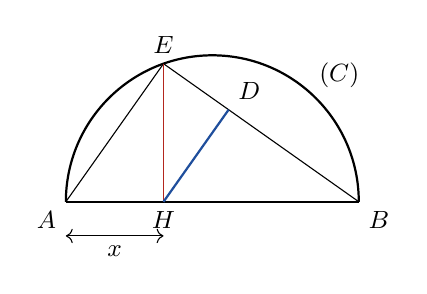
\begin{tikzpicture}[scale=0.62,font=\small]
\draw[thick] (6,0) arc (0:180:3);
\draw[thick] (0,0)--(6,0);
\coordinate (A) at (0,0); \coordinate (B) at (6,0); \coordinate (H) at (2,0);
\coordinate (E) at (2,2.828);
\draw (A)--(E)--(B); \draw[cThm] (E)--(H);
\coordinate (D) at ($(B)!(H)!(E)$);
\draw[cDef,thick] (H)--(D);
\node[below left] at (A){$A$}; \node[below right] at (B){$B$}; \node[below] at (H){$H$};
\node[above] at (E){$E$}; \node[above right] at (D){$D$};
\draw[<->] (0,-0.7)--(2,-0.7) node[midway,below]{$x$};
\node at (5.6,2.6){$(C)$};
\end{tikzpicture}
\end{LTR}\end{center}}
\end{tamrin}
\begin{hal}
\textbf{I) 1.} $g(x)=\dfrac{\sqrt6}{6}\,u(x)v(x)$ مع $u(x)=6-x$ ، $v(x)=\sqrt x$ ، $u'(x)=-1$ ، $v'(x)=\dfrac{1}{2\sqrt x}$:
\[g'(x)=\frac{\sqrt6}{6}\Big(-\sqrt x+\frac{6-x}{2\sqrt x}\Big)=\frac{\sqrt6}{6}\times\frac{-2x+6-x}{2\sqrt x}=\frac{\sqrt6}{6}\times\frac{3(2-x)}{2\sqrt x}=\bx{\frac{\sqrt6}{4}\times\frac{-x+2}{\sqrt x}}.\]
\QQ{2} $\dfrac{\sqrt6}{4}>0$ و $\sqrt x>0$ ، فإشارة $g'(x)$ هي إشارة $-x+2$:
\begin{TAB}
\tkzTabInit[lgt=1.3,espcl=2.6]{$x$/0.7,$g'(x)$/0.7,$g(x)$/1.4}{$0$,$2$,$6$}
\tkzTabLine{d,+,z,-,d}
\tkzTabVar{-/,+/$\frac{4\sqrt3}{3}$,-/}
\end{TAB}
$g(2)=\dfrac{\sqrt6}{6}\times4\times\sqrt2=\dfrac{4\sqrt{12}}{6}=\dfrac{8\sqrt3}{6}=\dfrac{4\sqrt3}{3}$.

\textbf{II) 1.} $H$ تختلف عن $A$ و $B$ ، إذن \bx{x\in\,]0;6[}.
\QQ{2} $E$ نقطة من نصف الدائرة التي قطرها $[AB]$ ، إذن المثلث $AEB$ \textbf{قائم في $E$} (كل مثلث محاط بدائرة وأحد أضلاعه قطر لها قائم).
\QQ{3} في $ABE$ القائم في $E$: $\cos\widehat{BAE}=\dfrac{AE}{AB}=\dfrac{AE}{6}$ ؛ \ في $AHE$ القائم في $H$: $\cos\widehat{BAE}=\dfrac{AH}{AE}=\dfrac{x}{AE}$.\par
إذن $\dfrac{AE}{6}=\dfrac{x}{AE}$ ، ومنه $AE^2=6x$ ، أي \bx{AE=\sqrt{6x}}.
\QQ{4} في $ABE$: $\sin\widehat{ABE}=\dfrac{AE}{AB}=\dfrac{\sqrt{6x}}{6}$ ؛ \ في $HDB$ القائم في $D$: $\sin\widehat{ABE}=\dfrac{HD}{HB}=\dfrac{HD}{6-x}$.\par
إذن $HD=\dfrac{\sqrt{6x}\,(6-x)}{6}=\dfrac{\sqrt6\sqrt x(6-x)}{6}$ ، أي \bx{h(x)=\dfrac{\sqrt6}{6}(6-x)\sqrt x=g(x)}.
\QQ{5} $h=g$ ، ومن جدول التغيرات: $HD$ أكبر ما يمكن من أجل \bx{x=2\ \text{cm}} ، وقيمتها العظمى $\dfrac{4\sqrt3}{3}\approx2{,}31\ \text{cm}$.
\end{hal}

% ------------------------------------------------- 20
\begin{tamrin}{أقصر مماس داخل مربع}
$ABCD$ مربع طول ضلعه $AB=2$. \ لتكن $(\Gamma)$ الدائرة التي مركزها $D$ ونصف قطرها $2$ ، و $M$ نقطة من القوس $\overset{\frown}{AC}$ تختلف عن $A$ و $C$. \ المماس $(T)$ للدائرة $(\Gamma)$ عند $M$ يقطع القطعة $[AB]$ في $K$ والقطعة $[BC]$ في $L$.\par
نريد تعيين وضعية $M$ حتى يأخذ الطول $KL$ أصغر قيمة ممكنة. نضع: $KB=x$ و $LB=y$.
\RL{0.6}{%
\textbf{1.} أثبت أن $KL^2=x^2+y^2$.\par
\textbf{2.} علماً أن $KA=KM$ و $LC=LM$ (مماسان من نقطة واحدة) ، أثبت أن $KL=4-x-y$ ، ثم استنتج أن:\\ $x^2+y^2=x^2+y^2-8x-8y+2xy+16$.\par
\textbf{3.} استنتج أن $y=\dfrac{4x-8}{x-4}$ ، ثم أن: $KL=\dfrac{-x^2+4x-8}{x-4}$.\par
\textbf{4.} لتكن $f$ الدالة المعرفة على $[0;2]$ بـ: $f(x)=\dfrac{-x^2+4x-8}{x-4}$. \ ادرس تغيرات $f$ ، واستنتج أن الطول $KL$ يأخذ أصغر قيمة ممكنة من أجل $x=4-2\sqrt2$.\par
\textbf{5.} عيّن عندئذ وضعية $M$.\par}
{0.37}{%
\begin{center}\begin{LTR}
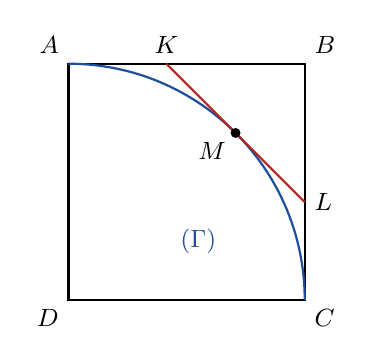
\begin{tikzpicture}[scale=1.5,font=\small]
\draw[thick] (0,0) rectangle (2,2);
\draw[cDef,thick] (2,0) arc (0:90:2);
\coordinate (D) at (0,0); \coordinate (A) at (0,2); \coordinate (B) at (2,2); \coordinate (C) at (2,0);
\coordinate (M) at (1.414,1.414);
\coordinate (K) at (0.828,2); \coordinate (L) at (2,0.828);
\draw[cThm,thick] (K)--(L);
\fill (M) circle(1.2pt);
\node[below left] at (D){$D$}; \node[above left] at (A){$A$}; \node[above right] at (B){$B$}; \node[below right] at (C){$C$};
\node[above] at (K){$K$}; \node[right] at (L){$L$}; \node[below left] at (M){$M$};
\node[cDef] at (1.1,0.5){$(\Gamma)$};
\end{tikzpicture}
\end{LTR}\end{center}}
\end{tamrin}
\begin{hal}
\textbf{1.} المثلث $KBL$ قائم في $B$ (زاوية المربع) ، وحسب فيثاغورث: \bx{KL^2=KB^2+BL^2=x^2+y^2}.
\QQ{2} $KL=KM+ML=KA+LC=(2-x)+(2-y)=\bx{4-x-y}$.\par
بالتربيع: $KL^2=(4-x-y)^2=16+x^2+y^2-8x-8y+2xy$ ، ومع السؤال 1: $x^2+y^2=x^2+y^2-8x-8y+2xy+16$.
\QQ{3} بالاختزال: $0=-8x-8y+2xy+16$ ، أي $y(2x-8)=8x-16$ ، ومنه ($x\ne4$): \bx{y=\dfrac{8x-16}{2x-8}=\dfrac{4x-8}{x-4}}.\par
\begin{align*}
KL&=4-x-\frac{4x-8}{x-4}\\
&=\frac{(4-x)(x-4)-(4x-8)}{x-4}=\frac{-x^2+8x-16-4x+8}{x-4}=\bx{\frac{-x^2+4x-8}{x-4}}.
\end{align*}
\QQ{4} $f'(x)=\dfrac{(-2x+4)(x-4)-(-x^2+4x-8)}{(x-4)^2}=\dfrac{-2x^2+12x-16+x^2-4x+8}{(x-4)^2}=\dfrac{-x^2+8x-8}{(x-4)^2}$.\par
$-x^2+8x-8=0$: $\Delta=64-32=32$ ، الجذران $4-2\sqrt2\approx1{,}17$ و $4+2\sqrt2$ (خارج $[0;2]$).\par
على $[0;2]$: $-x^2+8x-8<0$ قبل $4-2\sqrt2$ و $>0$ بعده:
\begin{TAB}
\tkzTabInit[lgt=1.3,espcl=2.6]{$x$/0.7,$f'(x)$/0.7,$f(x)$/1.4}{$0$,$4-2\sqrt2$,$2$}
\tkzTabLine{,-,z,+,}
\tkzTabVar{+/$2$,-/$4\sqrt2-4$,+/$2$}
\end{TAB}
$f(0)=\dfrac{-8}{-4}=2$ ، $f(2)=\dfrac{-4}{-2}=2$ ، و $f\big(4-2\sqrt2\big)=4\sqrt2-4\approx1{,}66$.\par
إذن $KL$ أصغر ما يمكن من أجل \bx{x=4-2\sqrt2} ، وقيمته الصغرى \bx{KL=4\sqrt2-4\approx1{,}66}.
\QQ{5} عندئذ $y=\dfrac{4(4-2\sqrt2)-8}{-2\sqrt2}=\dfrac{8-8\sqrt2}{-2\sqrt2}=4-2\sqrt2=x$ ، أي $KB=LB$: المثلث $KBL$ متساوي الساقين ، والمماس عمودي على القطر $[DB]$ ، إذن \textbf{$M$ هي نقطة تقاطع القوس مع القطر $[DB]$}.
\end{hal}

% ------------------------------------------------- 21
\begin{tamrin}{علبة بأكبر حجم}
لدينا قطعة من الورق المقوى مربعة الشكل طول ضلعها $12\ \text{cm}$. نقطع من أركانها الأربعة مربعات متقايسة طول ضلع كل منها $x$ (بالسنتيمتر) ، ثم نطوي الحواف لنحصل على علبة دون غطاء على شكل متوازي مستطيلات.
\begin{enumerate}
\item ما هي القيم الممكنة لـ $x$؟
\item بيّن أن حجم العلبة هو: $V(x)=x(12-2x)^2$.
\item ادرس تغيرات الدالة $V$ على المجال $]0;6[$.
\item استنتج قيمة $x$ التي يكون من أجلها حجم العلبة أكبر ما يمكن ، واحسب هذا الحجم.
\end{enumerate}
\end{tamrin}
\begin{hal}
\textbf{1.} يجب أن يكون $x>0$ و $12-2x>0$ ، إذن \bx{x\in\,]0;6[}.
\QQ{2} قاعدة العلبة مربع طول ضلعه $12-2x$ ، وارتفاعها $x$: \ $V(x)=(12-2x)^2\times x$.
\QQ{3} $V$ جداء $u=x$ و $v=(12-2x)^2$: \ $u'=1$ ، $v'=2\times(-2)(12-2x)=-4(12-2x)$:
\[V'(x)=(12-2x)^2-4x(12-2x)=(12-2x)(12-2x-4x)=(12-2x)(12-6x)=12(6-x)(2-x).\]
على $]0;6[$: $6-x>0$ ، فإشارة $V'(x)$ هي إشارة $2-x$:
\begin{TAB}
\tkzTabInit[lgt=1.3,espcl=2.6]{$x$/0.7,$V'(x)$/0.7,$V(x)$/1.4}{$0$,$2$,$6$}
\tkzTabLine{,+,z,-,}
\tkzTabVar{-/$0$,+/$128$,-/$0$}
\end{TAB}
\QQ{4} $V$ تبلغ قيمتها العظمى عند \bx{x=2\ \text{cm}} ، و $V(2)=2\times8^2=\bx{128\ \text{cm}^3}$.
\end{hal}

% ------------------------------------------------- 22
\begin{tamrin}{المقارنة والمتباينات بواسطة المشتقة}
\begin{enumerate}
\item نعتبر العددين:
\[A=\frac{(5{,}012013014015016)^2+3}{3{,}012013014015016}\qquad\text{\ar{و}}\qquad B=\frac{(5{,}012013014015017)^2+3}{3{,}012013014015017}.\]
باستعمال الدالة $f:x\mapsto\dfrac{x^2+3}{x-2}$ ، قارن بين $A$ و $B$.
\item باستعمال دراسة دالة مناسبة ، بيّن أنه:
\begin{sq}
\qa من أجل كل عدد حقيقي $x\ge0$: $\sin x\le x$.
\qb من أجل كل عدد حقيقي $x\ge0$: $\sqrt{1+x}\le1+\dfrac x2$.
\end{sq}
\end{enumerate}
\end{tamrin}
\begin{hal}
\textbf{1.} نضع $x_1=5{,}012013014015016$ و $x_2=5{,}012013014015017$: \ $x_1-2=3{,}012\ldots016$ ، إذن $A=f(x_1)$ و $B=f(x_2)$.\par
$f'(x)=\dfrac{2x(x-2)-(x^2+3)}{(x-2)^2}=\dfrac{x^2-4x-3}{(x-2)^2}$. \ $x^2-4x-3=0$: $\Delta=28$ ، الجذران $2-\sqrt7$ و $2+\sqrt7\approx4{,}65$.\par
على $\big[2+\sqrt7;+\infty\big[$: $f'(x)\ge0$ ، فـ $f$ متزايدة تماماً. \ $x_1$ و $x_2$ ينتميان إلى هذا المجال (لأنهما أكبر من $4{,}65$) و $x_1<x_2$ ، إذن $f(x_1)<f(x_2)$: \ \bx{A<B}.

\QQ{2} \pa نضع $\varphi(x)=x-\sin x$ على $[0;+\infty[$: \ $\varphi'(x)=1-\cos x\ge0$ (لأن $\cos x\le1$).\par
إذن $\varphi$ متزايدة على $[0;+\infty[$ ، ومنه من أجل $x\ge0$: $\varphi(x)\ge\varphi(0)=0$ ، أي $x-\sin x\ge0$: \ \bx{\sin x\le x}.
\pb نضع $\psi(x)=1+\dfrac x2-\sqrt{1+x}$ على $[0;+\infty[$: \ $\psi'(x)=\dfrac12-\dfrac{1}{2\sqrt{1+x}}=\dfrac{\sqrt{1+x}-1}{2\sqrt{1+x}}$.\par
من أجل $x\ge0$: $\sqrt{1+x}\ge1$ ، إذن $\psi'(x)\ge0$ و $\psi$ متزايدة ، ومنه $\psi(x)\ge\psi(0)=1-1=0$: \ \bx{\sqrt{1+x}\le1+\dfrac x2}.\par
\textbf{تفسير بياني:} منحنى $x\mapsto\sqrt{1+x}$ يقع تحت مماسه $y=1+\dfrac x2$ عند النقطة ذات الفاصلة $0$.
\end{hal}

\end{document}
